% Rapport de projet – modèle de rapport de l'École Centrale Casablanca
% Compilation : tectonic main.tex   (ou xelatex + bibtex sur Overleaf)
\documentclass[11pt,a4paper]{article}

% ---------------------------------------------------------------- Langue, polices
\usepackage{fontspec}
\usepackage[french]{babel}
\usepackage{csquotes}

% ---------------------------------------------------------------- Mise en page
\usepackage[a4paper,top=2.5cm,bottom=2.5cm,left=2.5cm,right=2.5cm,headheight=14pt]{geometry}
\usepackage{fancyhdr}
\usepackage{graphicx}
\usepackage{tikz}
\usepackage{eso-pic}
\usepackage{xcolor}
\usepackage{float}
\usepackage{caption}
\usepackage{subcaption}
\usepackage{booktabs}
\usepackage{tabularx}
\usepackage{multirow}
\usepackage{array}
\usepackage{enumitem}
\usepackage{amsmath,amssymb}
\usepackage{siunitx}
\usepackage[hidelinks]{hyperref}

\sisetup{output-decimal-marker={,},group-separator={\,}}
\graphicspath{{../figures/}{images/}}
\setlist{itemsep=2pt,topsep=4pt}
\captionsetup{labelsep=endash,font=small}
\definecolor{centrale}{HTML}{00966C}

% ---------------------------------------------------------------- Bibliographie
\usepackage[backend=bibtex,style=numeric,sorting=nyt,maxbibnames=4]{biblatex}
\renewcommand*{\mkbibnamefamily}[1]{\textsc{#1}}
\addbibresource{references.bib}
\catcode"200B=9 % espace de largeur nulle (biblatex en français) : ignorée

% ---------------------------------------------------------------- Informations du rapport
\newcommand{\titre}{Assistant multi-agent pour la sélection intelligente de portefeuilles financiers}
\newcommand{\titrecourt}{Assistant multi-agent de portefeuille}
\newcommand{\matiere}{Introduction aux techniques d'apprentissage automatique}

% ---------------------------------------------------------------- En-têtes et pieds de page
\pagestyle{fancy}
\fancyhf{}
\renewcommand{\sectionmark}[1]{\markboth{}{\thesection\quad #1}}
\renewcommand{\subsectionmark}[1]{}
\newcolumntype{L}{>{\raggedright\arraybackslash}X}
\fancyhead[L]{\textit{\leftmark}}
\fancyhead[R]{\rightmark}
\fancyfoot[C]{Rapport - \textbf{\titrecourt}}
\fancyfoot[R]{\thepage}
\renewcommand{\headrulewidth}{0.4pt}

\begin{document}

% ================================================================ Page de garde
\pagenumbering{Alph}
\begin{titlepage}
  \AddToShipoutPictureBG*{%
    \AtPageLowerLeft{\put(\LenToUnit{0.47\paperwidth},\LenToUnit{0.03\paperheight}){%
      
\includegraphics[height=0.56\paperheight]{fond_garde.jpg}}}}
  \centering
  \vspace*{1.2cm}
  
\includegraphics[width=0.42\textwidth]{logo_centrale.jpg}\par
  \vspace{1.6cm}
  {\Large\scshape École Centrale Casablanca\par}
  \vspace{1.4cm}
  {\large\scshape \matiere\par Rapport de projet\par}
  \vspace{1.2cm}
  \rule{\linewidth}{0.5pt}\par\vspace{0.4cm}
  {\LARGE\bfseries \titre\par}
  \vspace{0.3cm}\rule{\linewidth}{0.5pt}\par
  \vspace{2cm}
  \begin{minipage}[t]{0.55\textwidth}
    \raggedright
    \textbf{\textit{Élèves :}}\\
    Wendin Naandé Alain \textsc{Kissou}\\
    Mory Désiré \textsc{Ouattara}\\
    Mahamoudou \textsc{Ouedraogo}\\
    Mouhamadou Bachir \textsc{Ngom}
  \end{minipage}%
  \begin{minipage}[t]{0.4\textwidth}
    \raggedleft
    \vspace{0.4cm}
    \textbf{\textit{Encadrant :}}\\
    Pr. Y. \textsc{Lamrani Alaoui}
  \end{minipage}
  \vfill
  {\large 30 novembre 2026\par}
\end{titlepage}

% ================================================================ Table des matières
\pagenumbering{arabic}
\markboth{TABLE DES MATIÈRES}{Table des matières}
\tableofcontents
\clearpage

% ================================================================ Corps du rapport
\section{Introduction}
\label{sec:introduction}

\subsection{Contexte}

Proposer un placement à un client est un exercice à trois volets. Il faut d'abord \emph{connaître le client} : son horizon, sa situation financière, sa capacité réelle à supporter une perte. Il faut ensuite \emph{lire le marché} : une même allocation n'a pas le même risque dans une période calme et au cœur d'une crise. Il faut enfin \emph{justifier} la recommandation, ce que la réglementation impose aux conseillers et ce que le client est en droit d'attendre.

L'apprentissage automatique semble bien armé pour chacun de ces volets : classer des clients à partir de leurs caractéristiques, repérer des états de marché, prévoir des rendements. La littérature appelle pourtant à la prudence. La prévision des rendements financiers est notoirement difficile : la plupart des variables proposées ne battent pas, hors échantillon, une simple moyenne historique~\cite{welch2008}, et les gains obtenus par l'apprentissage automatique restent modestes même avec des données très riches~\cite{gu2020}. De même, les portefeuilles optimisés battent rarement la règle naïve qui répartit le capital à parts égales~\cite{demiguel2009}. Enfin, les données financières se prêtent à des erreurs méthodologiques, les \emph{fuites de données}, qui produisent des performances spectaculaires sur le papier et décevantes en réalité~\cite{lopezdeprado2018}.

\subsection{Problématique et objectifs}

Notre problématique est la suivante : \emph{comment construire un assistant qui recommande à chaque client un portefeuille adapté à son profil et à l'état du marché, explique sa recommandation, et dont on puisse mesurer honnêtement la valeur ?}

Nous nous sommes fixé quatre objectifs :
\begin{enumerate}
  \item \textbf{Couvrir les familles de méthodes du cours}~\cite{cours_ml} sur un problème réel : apprentissage supervisé (classification et régression), non supervisé (clustering, détection d'anomalies), réduction de dimension, apprentissage par renforcement et interprétabilité.
  \item \textbf{Évaluer sans fuite de données}, avec des références simples (\emph{baselines}) et des tests statistiques, et accepter les conclusions négatives.
  \item \textbf{Rendre chaque décision explicable}, au niveau global (quelles variables comptent) et au niveau d'un client (pourquoi ce profil, pourquoi ce portefeuille).
  \item \textbf{Livrer un outil utilisable} : une application web que l'on peut essayer en ligne ou réinstaller à partir du dépôt.
\end{enumerate}

\subsection{Approche : un système multi-agent}

Plutôt qu'un modèle unique, nous avons découpé le problème en tâches confiées à des \emph{agents} spécialisés~\cite{wooldridge2009}. Chaque agent répond à une seule question avec la famille de méthodes la plus adaptée (tableau~\ref{tab:agents}). Les agents communiquent par un \emph{tableau noir} partagé, et un orchestrateur les appelle dans l'ordre, avec une boucle de négociation entre l'agent Allocation et l'agent Risque (figure~\ref{fig:architecture}).

\begin{table}[H]
  \centering
  \small
  \caption{Les sept agents, la question qu'ils traitent et les méthodes comparées.}
  \label{tab:agents}
  \begin{tabularx}{\textwidth}{@{}l L l L@{}}
    \toprule
    \textbf{Agent} & \textbf{Question traitée} & \textbf{Paradigme} & \textbf{Méthodes comparées} \\
    \midrule
    Profil      & Le client peut-il supporter des pertes ? & Classification & Logistique, KNN, SVM, arbre, forêt, boosting, MLP ; SMOTE, ADASYN \\
    Prévision   & Quels actifs surperformeront le mois prochain ? & Régression temporelle & MCO, Ridge, Lasso, Elastic Net, KNN, SVR, arbres, boosting, MLP ; ACP \\
    Régime      & Le marché est-il calme ou stressé ? & Clustering & K-means, CAH, DBSCAN, mélange gaussien \\
    Alerte      & La journée est-elle anormale ? & Anomalies & z-score, Grubbs, gaussienne, Isolation Forest, LOF, One-Class SVM \\
    Risque      & Quel est le risque du portefeuille ? & Statistique & Ledoit-Wolf, VaR, CVaR \\
    Allocation  & Quel portefeuille choisir ? & Optimisation, renforcement & Moyenne-variance (Black-Litterman), parité de risque, HRP, PPO \\
    Explication & Pourquoi cette recommandation ? & Interprétabilité & Coefficients, permutation, SHAP \\
    \bottomrule
  \end{tabularx}
\end{table}

\begin{figure}[H]
  \centering
  \begin{tikzpicture}[
      font=\small,
      src/.style={draw=gray!60, fill=gray!8, rounded corners=3pt, minimum width=2.9cm, minimum height=0.85cm, align=center},
      ag/.style={draw=black!70, rounded corners=3pt, minimum width=3.3cm, minimum height=0.85cm, align=center},
      fl/.style={-latex, thick, gray!70!black}]
    % Sources
    \node[src] (s1) at (0, 3.0) {Formulaire client};
    \node[src] (s2) at (0, 1.8) {Marchés (FRED, Yahoo)};
    \node[src] (s3) at (0, 0.6) {Marchés (rendements)};
    \node[src] (s4) at (0,-0.6) {Panel de 25 actifs};
    \node[src] (s5) at (0,-1.8) {Cours sur 1 an};
    % Agents d'analyse
    \node[ag, fill=blue!10]   (pr) at (4, 3.0) {\textbf{Profil}\\ régression logistique};
    \node[ag, fill=green!10]  (re) at (4, 1.8) {\textbf{Régime}\\ mélange gaussien};
    \node[ag, fill=orange!12] (al) at (4, 0.6) {\textbf{Alerte}\\ vote de 4 détecteurs};
    \node[ag, fill=yellow!15] (pv) at (4,-0.6) {\textbf{Prévision}\\ ensemble (non activé)};
    \node[ag, fill=red!10]    (ri) at (4,-1.8) {\textbf{Risque}\\ Ledoit-Wolf, VaR};
    % Tableau noir
    \node[ag, fill=purple!10, minimum height=5.6cm, minimum width=2.2cm] (bb) at (7.6, 0.6) {\textbf{Tableau}\\ \textbf{noir}\\ partagé};
    % Décision
    \node[ag, fill=cyan!10]   (alc) at (11.3, 2.2) {\textbf{Allocation}\\ moyenne-variance};
    \node[ag, fill=red!10]    (ctl) at (11.3, 0.6) {\textbf{Risque}\\ contrôle des limites};
    \node[ag, fill=violet!10] (ex)  at (11.3,-1.0) {\textbf{Explication}\\ texte + SHAP};
    \node[align=center, font=\small\bfseries] (out) at (11.3,-2.3) {Recommandation justifiée};
    \foreach \a/\b in {s1/pr, s2/re, s3/al, s4/pv, s5/ri} \draw[fl] (\a) -- (\b);
    \foreach \a in {pr, re, al, pv, ri} \draw[fl] (\a.east) -- (bb.west |- \a.east);
    \draw[fl] (bb.east |- alc.west) -- (alc.west);
    \draw[fl] (alc.south) ++(-0.4,0) -- ++(0,-0.75);
    \draw[fl, red!70!black] (ctl.north) ++(0.4,0) -- ++(0,0.75) node[midway, right, font=\scriptsize, align=left] {renégociation\\si limite dépassée};
    \draw[fl] (ctl) -- (ex);
    \draw[fl] (ex) -- (out);
  \end{tikzpicture}
  \caption{Architecture du système. Les agents d'analyse déposent leurs conclusions sur le tableau noir ; l'agent Allocation propose un portefeuille que l'agent Risque accepte ou renvoie avec une contrainte plus stricte ; l'agent Explication rédige la recommandation.}
  \label{fig:architecture}
\end{figure}

Ce découpage a trois avantages. Chaque agent peut être évalué \emph{séparément}, avec la métrique et la référence qui lui conviennent. Un agent qui n'apporte rien peut être \emph{désactivé} sans toucher aux autres : c'est ce qui arrive à l'agent Prévision (section~\ref{sec:prevision}). Enfin, la chaîne de décision est \emph{lisible} : le journal des échanges sur le tableau noir montre qui a décidé quoi.

\subsection{Démarche}

Nous avons suivi pour chaque agent le processus de développement présenté en cours : compréhension du problème, collecte et nettoyage des données, analyse exploratoire, préparation, séparation entraînement / validation / test, entraînement, évaluation, optimisation des hyperparamètres, puis déploiement. Une règle traverse tout le projet : \textbf{la période de test ne sert à aucun choix}. Tous les réglages (modèle retenu, seuils, hyperparamètres, paramètres de l'allocation) sont fixés sur la validation, et le test sert à une évaluation unique.

L'ensemble est reproductible : un notebook unique, organisé dans le même ordre que ce rapport, s'exécute de bout en bout en 22 minutes et produit tous les tableaux et figures cités. Le code, les données et les modèles sont publiés sur GitHub\footnote{\url{https://github.com/kissou-alain/Assistant-Portefeuille-financier}}, et l'application est accessible en ligne\footnote{\url{https://assistant-portefeuille-financier.vercel.app}}.

\subsection{Organisation du rapport}

La section~\ref{sec:donnees} présente les données et le protocole qui empêche les fuites. Les sections~\ref{sec:profil} à~\ref{sec:regime_alerte} détaillent les agents d'apprentissage : Profil (classification), Prévision (régression temporelle), Régime et Alerte (non supervisé). La section~\ref{sec:systeme} décrit leur assemblage, la section~\ref{sec:allocation_backtest} l'allocation et son évaluation historique, et la section~\ref{sec:renforcement} l'alternative par renforcement. La section~\ref{sec:application} présente l'application. Nous discutons enfin la pertinence de la démarche, sa valeur ajoutée et ses limites (section~\ref{sec:discussion}), avant de conclure sur les perspectives et sur ce que ce projet nous a appris (section~\ref{sec:conclusion}).

\section{Données, prétraitement et prévention des fuites}
\label{sec:donnees}

À rédiger.

\section{Agent Profil : estimer la capacité à prendre des risques}
\label{sec:profil}

À rédiger.

\section{Agent Prévision : prévoir les rendements, et savoir y renoncer}
\label{sec:prevision}

\subsection{Formulation : une régression sur données temporelles}

L'agent Prévision cherche à repérer les actifs qui feront mieux que les autres le mois suivant. Pour chaque actif $i$ et chaque date $t$, la cible est le rendement \emph{excédentaire} sur $H = 21$ jours de bourse :
\begin{equation}
  y_{i,t} = r_{i,\,t\to t+H} - \frac{1}{N_t}\sum_{j=1}^{N_t} r_{j,\,t\to t+H}.
\end{equation}
Retirer la moyenne des actifs supprime l'effet \og marché \fg{} commun, que l'allocation n'a pas besoin de prévoir : seul compte le classement relatif. La cible a un écart-type de 5,1 \% par mois sur l'entraînement.

Les données sont organisées par \textbf{fenêtre glissante}, comme le présente le cours pour les données temporelles (tableau~\ref{tab:fenetre}). À chaque date, les 31 variables de la section~\ref{sec:donnees} résument le passé, et la cible porte sur l'horizon futur.

\begin{table}[!htb]
  \centering
  \small
  \caption{Paramètres de la fenêtre glissante.}
  \label{tab:fenetre}
  \begin{tabularx}{\textwidth}{@{}l L L@{}}
    \toprule
    \textbf{Terme} & \textbf{Définition} & \textbf{Valeur dans le projet} \\
    \midrule
    \emph{Lookback} $L$ & Nombre de pas passés utilisés en entrée & 252 jours (la variable la plus longue porte sur un an) \\
    \emph{Forecast horizon} $H$ & Nombre de pas futurs à prédire & 21 jours, prévision directe \\
    \emph{Stride} $S$ & Décalage entre deux échantillons & 5 jours (un échantillon par semaine) \\
    \emph{Input size} & Variables par pas de temps & 31 \\
    Chevauchement & Échantillons dont les cibles se recouvrent & $\lceil H/S\rceil - 1 = 4$ \\
    \bottomrule
  \end{tabularx}
\end{table}

Le choix du \emph{stride} est un compromis. Avec $S = 1$, deux échantillons consécutifs partageraient 20 jours de cible sur 21 : ce seraient presque des doublons, qui donneraient une fausse impression de quantité de données. Avec $S = 21$, il ne resterait qu'environ 110 dates d'entraînement. Avec $S = 5$, le chevauchement résiduel de quatre échantillons est pris en compte dans les tests statistiques (correction de Newey-West~\cite{newey1987} et test de Diebold-Mariano). Le panel compte 98\,716 observations ; après découpage et purge, l'entraînement couvre 449 dates (2011-2019), la validation 96 (2020-2021) et le test 241 (janvier 2022 à octobre 2026).

\subsection{Analyse exploratoire du pouvoir prédictif}

En gestion d'actifs, on mesure le pouvoir prédictif d'une variable par son \textbf{coefficient d'information} (IC) : la corrélation de rang de Spearman entre la variable et le rendement futur, calculée date par date puis moyennée. Un IC de 0,03 à 0,05, s'il est stable, est déjà considéré comme exploitable.

Sur l'entraînement, la médiane des IC en valeur absolue n'est que de 0,04. Les variables les plus liées au rendement futur sont la corrélation au S\&P~500 (0,15), le bêta (0,12) et la volatilité (0,07), toutes de signe positif. Elles ne repèrent pas les bons actifs \emph{au sein} d'une classe : elles distinguent les actions des obligations. De 2011 à 2019, marché haussier, les actifs risqués ont nettement battu les actifs défensifs. Ce \og signal \fg{} est une \emph{prime de classe d'actifs propre à la période d'entraînement}. Si le contexte change, il peut disparaître : c'est un risque de \textbf{dérive des données} (\emph{data drift}), et c'est ce qui se produira en 2022.

L'analyse montre aussi que les variables techniques sont fortement corrélées entre elles : différents horizons de momentum, différentes mesures de volatilité. Deux conséquences en découlent : il faudra des modèles régularisés, et une réduction de dimension peut être envisagée.

\subsection{Réduction de dimension : analyse en composantes principales}

L'ACP remplace des variables corrélées par des combinaisons linéaires non corrélées, les composantes principales $F_k = X V_k$, où les $V_k$ sont les vecteurs propres de la matrice de covariance des variables standardisées, rangés par valeur propre $\lambda_k$ décroissante. La part de variance expliquée par $F_k$ vaut $\lambda_k/\sum_j \lambda_j$.

Le cours rappelle que l'ACP n'a d'intérêt que si les variables sont suffisamment corrélées. Nous l'avons vérifié sur l'entraînement : l'indice KMO~\cite{kaiser1974} vaut 0,746 (au-dessus du seuil de 0,6) et le test de sphéricité de Bartlett est très significatif ($\chi^2 = 254\,994$, 190 degrés de liberté, $p < 10^{-4}$). L'ACP est donc justifiée.

\begin{figure}[!htb]
  \centering
  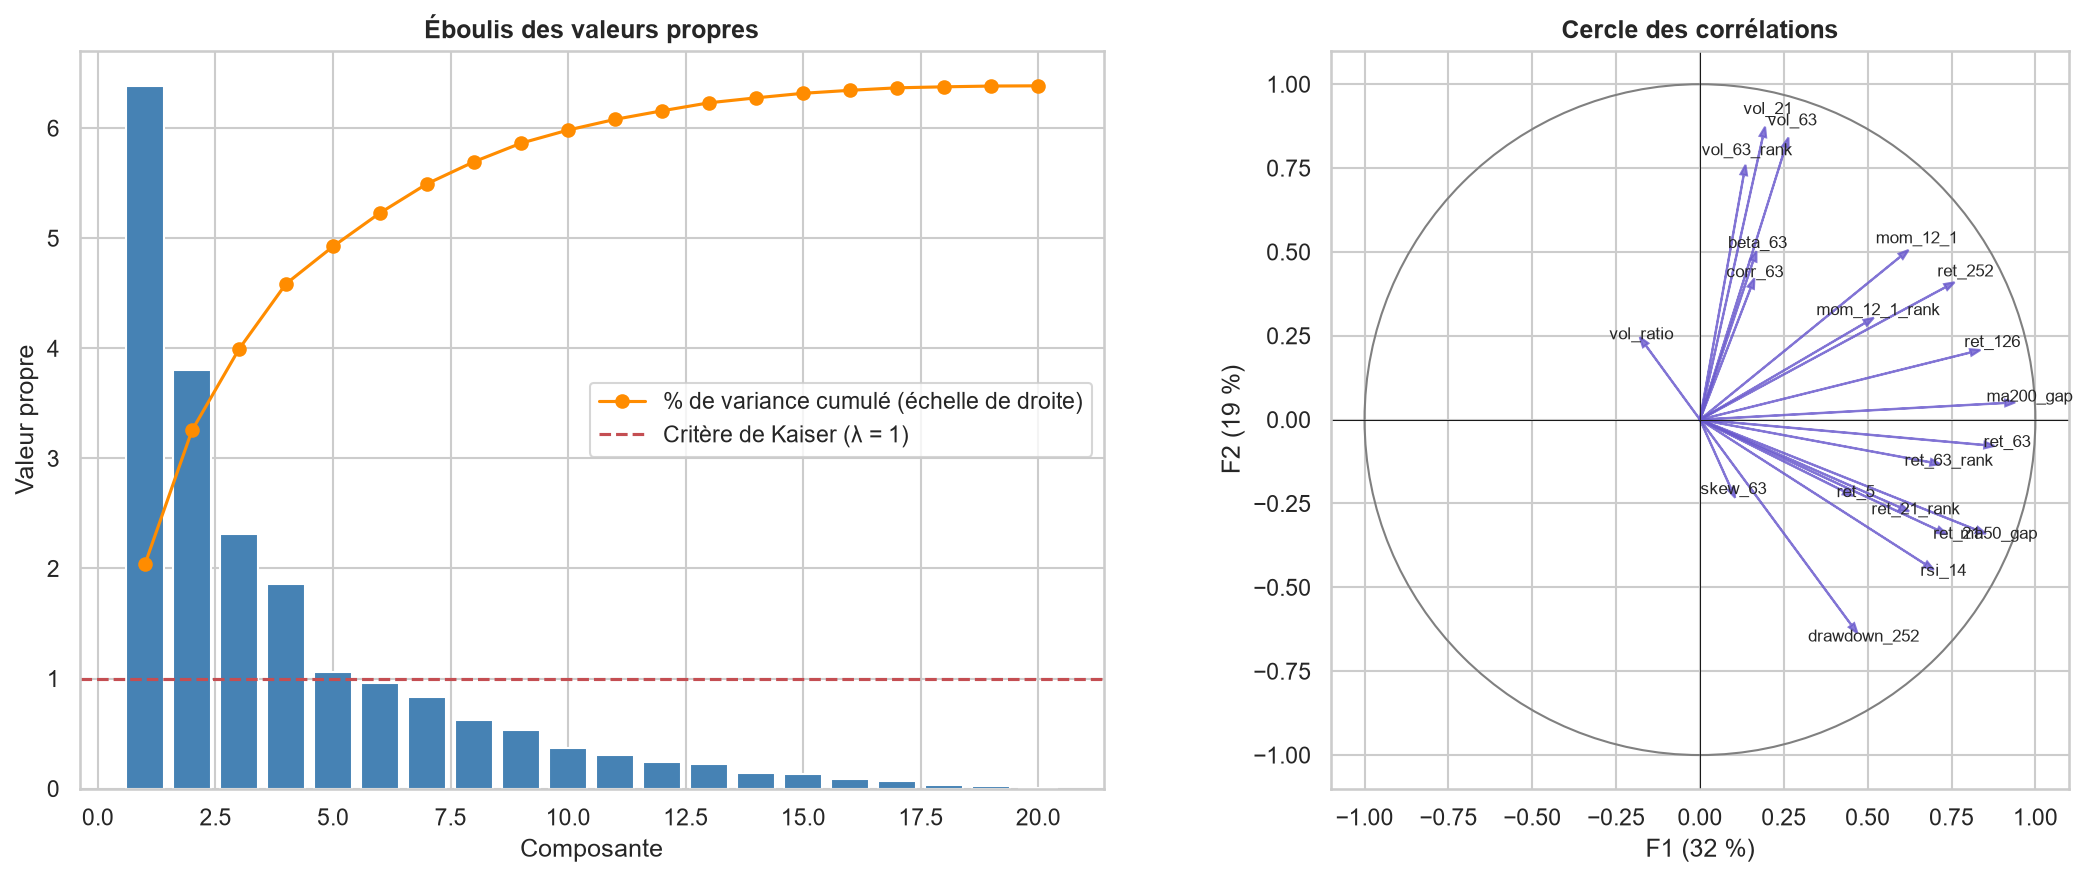
\includegraphics[width=\textwidth]{10b_acp.png}
  \caption{ACP des 20 variables techniques (entraînement) : éboulis des valeurs propres et cercle des corrélations sur le premier plan factoriel.}
  \label{fig:acp}
\end{figure}

Les deux premières composantes expliquent 51 \% de la variance, les cinq premières 77 \% (figure~\ref{fig:acp}). Elles ont une lecture financière claire :
\begin{itemize}
  \item \textbf{F1, \og tendance \fg{}} (32 \%) : corrélée à tous les rendements passés et aux écarts aux moyennes mobiles ;
  \item \textbf{F2, \og risque \fg{}} (19 \%) : corrélée aux volatilités, elle oppose les actifs agités aux actifs calmes ;
  \item \textbf{F3, \og retournement \fg{}} (12 \%) : elle oppose le momentum long au momentum court ;
  \item \textbf{F4, \og sensibilité au marché \fg{}} (9 \%) : corrélée au bêta et à la corrélation au S\&P~500.
\end{itemize}
Les critères de choix du nombre de composantes ne s'accordent pas : 2 selon le coude, 5 selon Kaiser ($\lambda \geq 1$), 6 pour 80 \% de variance, 9 pour 90 \%. Plutôt que de trancher a priori, nous testerons les modèles avec et sans ACP dans le pipeline.

\subsection{Références et modèles comparés}

Toute méthode doit faire mieux que des \textbf{références} sans apprentissage :
\begin{itemize}
  \item la \textbf{prévision nulle}, $\hat y = 0$ : aucun actif ne fera mieux que la moyenne ;
  \item la \textbf{moyenne historique par actif} : le rendement excédentaire moyen de chaque actif sur l'entraînement ;
  \item le \textbf{momentum 12-1} : les gagnants des douze derniers mois (hors le dernier) continuent de gagner.
\end{itemize}

Treize modèles du cours ont été comparés, tous dans un pipeline de prétraitement : régression linéaire (MCO) ; Ridge, Lasso et Elastic Net, qui ajoutent à l'erreur quadratique une pénalité $\lambda\lVert\beta\rVert_2^2$, $\lambda\lVert\beta\rVert_1$ ou un mélange des deux ; KNN ; SVR à noyau gaussien ; arbre de décision ; forêt aléatoire ; quatre algorithmes de \emph{boosting} (Gradient Boosting, LightGBM, XGBoost, CatBoost) ; MLP entraîné par Adam. Les hyperparamètres sont choisis par recherche aléatoire (10 combinaisons au plus) en \textbf{validation croisée temporelle à fenêtre croissante, purgée}, sur l'entraînement, selon l'erreur quadratique. Ils sont ensuite réutilisés tels quels dans toutes les comparaisons. La SVR, la plus coûteuse, est entraînée sur 3\,000 lignes.

\begin{table}[!htb]
  \centering
  \small
  \caption{Comparaison sur la validation 2020-2021 (96 dates). $R^2_{oos}$ : $R^2$ hors échantillon par rapport à la prévision nulle.}
  \label{tab:prev_val}
  \begin{tabular}{@{}l l r r r@{}}
    \toprule
    \textbf{Modèle} & \textbf{Famille} & \textbf{RMSE} & $\boldsymbol{R^2_{oos}}$ & \textbf{IC moyen} \\
    \midrule
    Moyenne par actif (référence) & Référence & 0,0691 & 8,4 \% & 0,196 \\
    Elastic Net & Linéaire régularisé & 0,0707 & 4,1 \% & 0,163 \\
    Ridge & Linéaire régularisé & 0,0709 & 3,6 \% & 0,157 \\
    XGBoost & \emph{Boosting} & 0,0710 & 3,4 \% & 0,159 \\
    LightGBM & \emph{Boosting} & 0,0712 & 2,9 \% & 0,126 \\
    Forêt aléatoire & \emph{Bagging} & 0,0714 & 2,3 \% & 0,162 \\
    Gradient Boosting & \emph{Boosting} & 0,0715 & 2,2 \% & 0,098 \\
    Arbre de décision & Arbre & 0,0717 & 1,5 \% & 0,115 \\
    Régression linéaire (MCO) & Linéaire & 0,0717 & 1,4 \% & 0,023 \\
    KNN & Voisinage & 0,0719 & 1,1 \% & 0,078 \\
    Momentum 12-1 (référence) & Référence & 0,0721 & 0,3 \% & 0,014 \\
    Prévision nulle (référence) & Référence & 0,0722 & 0 & -- \\
    Lasso & Linéaire régularisé & 0,0722 & 0,0 \% & -- \\
    SVR (noyau RBF) & Noyau & 0,0724 & $-0{,}4$ \% & $-0{,}005$ \\
    CatBoost & \emph{Boosting} & 0,0729 & $-1{,}8$ \% & 0,129 \\
    MLP (Adam) & Réseau & 0,0759 & $-10{,}4$ \% & 0,217 \\
    \bottomrule
  \end{tabular}
\end{table}

\paragraph{Interprétation.} Sur la validation (tableau~\ref{tab:prev_val}), le meilleur \og modèle \fg{} est une référence : la moyenne historique par actif. Les meilleurs modèles appris (Elastic Net, Ridge, XGBoost, forêt aléatoire) obtiennent un $R^2$ de 2 à 4 \% et un IC de 0,13 à 0,16. Les modèles les plus flexibles (MLP, SVR, CatBoost) font moins bien que la prévision nulle : avec un signal aussi faible, leur variance domine. Le cas du MLP est instructif : il a le meilleur IC (0,217) mais le pire $R^2$ ($-10$~\%). Il \emph{classe} bien les actifs sur cette période, mais ses prévisions sont beaucoup trop amples. Les deux métriques mesurent des choses différentes, et une seule période de deux ans ne permet pas de savoir si ce bon classement est durable. Les hyperparamètres retenus le confirment : régularisation maximale pour Ridge ($\lambda \approx 31\,600$), 500 voisins pour le KNN, arbres de profondeur 2 avec au moins 500 observations par feuille, $C = 0{,}01$ pour la SVR. La validation croisée pousse systématiquement vers les modèles les plus simples possibles.

\paragraph{Le Lasso choisit de ne rien prédire.} Le chemin de régularisation du Lasso (en annexe, figure~\ref{fig:lasso}) est particulièrement parlant. Quand $\lambda$ augmente, la pénalité $\lVert\beta\rVert_1$ ramène les coefficients exactement à zéro un par un : c'est une sélection de variables. La validation croisée retient un $\lambda$ pour lequel \emph{les 36 coefficients sont nuls}. Le meilleur Lasso est donc la prévision nulle : d'après la validation croisée, aucune variable n'apporte assez d'information pour mériter un coefficient. C'est un résultat, pas une panne.

\paragraph{L'ACP ne change presque rien.} En ajoutant au pipeline une ACP qui conserve 90 \% de la variance (15 composantes sur les variables numériques), Elastic Net et Ridge obtiennent quasiment les mêmes résultats ($R^2$ de 4,0 \% au lieu de 4,1 \% ; IC de 0,161 au lieu de 0,163). C'est cohérent : les modèles régularisés gèrent déjà les variables corrélées, la pénalité Ridge agissant comme une ACP \og douce \fg{} qui réduit surtout les directions de faible variance~\cite{hastie2009}. L'ACP a ici une valeur d'\emph{interprétation} (les quatre facteurs ci-dessus) plus que de performance.

\paragraph{Diagnostic biais-variance.} Pour Elastic Net, l'erreur d'entraînement ($J_{train} = 0{,}00179$) est nettement inférieure à l'erreur de validation croisée ($J_{cv} = 0{,}00279$), qui dépasse même celle de la prévision nulle (0,00261). Malgré une forte régularisation, le modèle apprend du bruit : nous sommes dans un régime de variance, où le signal est trop faible par rapport au bruit.

\subsection{Trois méthodes d'évaluation}

Les résultats précédents reposent sur une seule période de validation de deux ans. Le cours présente trois manières d'évaluer un modèle sur données temporelles ; nous les avons appliquées avec les mêmes hyperparamètres, sur 2011-2021, sans toucher au test :
\begin{enumerate}
  \item \textbf{\emph{hold-out} temporel} : apprentissage sur 2011-2019, évaluation sur 2020-2021 ;
  \item \textbf{validation croisée à fenêtre croissante} (\emph{expanding window}) : cinq plis, la fenêtre d'apprentissage s'allonge à chaque pli ;
  \item \textbf{validation croisée à fenêtre glissante} (\emph{rolling window}) : mêmes blocs d'évaluation, mais la fenêtre d'apprentissage garde une taille fixe.
\end{enumerate}

\begin{table}[!htb]
  \centering
  \small
  \caption{Les trois méthodes d'évaluation (mêmes hyperparamètres). IC : moyenne et écart-type entre plis.}
  \label{tab:trois_eval}
  \begin{tabular}{@{}l l r r r@{}}
    \toprule
    \textbf{Modèle} & \textbf{Méthode} & $\boldsymbol{R^2_{oos}}$ & \textbf{IC moyen} & \textbf{Écart-type IC} \\
    \midrule
    \multirow{3}{*}{Moyenne par actif} & \emph{Hold-out} & 8,4 \% & 0,196 & -- \\
     & Fenêtre croissante & $-3{,}0$ \% & 0,117 & 0,087 \\
     & Fenêtre glissante & $-8{,}7$ \% & 0,046 & 0,038 \\
    \midrule
    \multirow{3}{*}{Elastic Net} & \emph{Hold-out} & 4,1 \% & 0,163 & -- \\
     & Fenêtre croissante & $-1{,}7$ \% & 0,035 & 0,155 \\
     & Fenêtre glissante & $-4{,}8$ \% & $-0{,}006$ & 0,140 \\
    \midrule
    \multirow{3}{*}{Ridge} & \emph{Hold-out} & 3,6 \% & 0,157 & -- \\
     & Fenêtre croissante & $-0{,}1$ \% & 0,041 & 0,176 \\
     & Fenêtre glissante & $-0{,}6$ \% & $-0{,}015$ & 0,148 \\
    \midrule
    \multirow{3}{*}{XGBoost} & \emph{Hold-out} & 3,4 \% & 0,159 & -- \\
     & Fenêtre croissante & $-3{,}4$ \% & 0,043 & 0,179 \\
     & Fenêtre glissante & $-7{,}4$ \% & $-0{,}021$ & 0,144 \\
    \bottomrule
  \end{tabular}
\end{table}

Le tableau~\ref{tab:trois_eval} se lit avec la grille du cours, et chaque cas de cette grille s'y retrouve :
\begin{itemize}
  \item \textbf{Le \emph{hold-out} seul était trop optimiste.} Tous les modèles ont un $R^2$ positif sur 2020-2021, mais négatif ou nul en validation croisée, et leur IC s'effondre (de 0,16 à environ 0,04 pour Ridge). Un découpage unique, tombé sur une période favorable, aurait fait croire à un modèle prédictif. C'est sans doute l'enseignement méthodologique le plus important de ce projet.
  \item \textbf{La fenêtre croissante bat la fenêtre glissante} pour tous les modèles : l'historique long apporte de l'information utile, et une mémoire courte dégrade la prévision.
  \item \textbf{Les modèles sont instables} : l'écart-type de l'IC entre plis (0,14 à 0,18) dépasse largement sa moyenne. Le signe même du pouvoir prédictif change d'une période à l'autre.
\end{itemize}

\subsection{Test de Diebold-Mariano}

Pour affirmer qu'un modèle est meilleur qu'un autre, une erreur légèrement plus faible ne suffit pas : l'écart doit être statistiquement significatif. Le test de Diebold-Mariano~\cite{diebold1995} compare deux séries de prévisions. À chaque date $t$, on calcule le différentiel de perte $d_t = L(e_{1,t}) - L(e_{2,t})$, où $L$ est l'erreur quadratique moyenne sur les 25 actifs. On teste $H_0 : \mathbb{E}[d_t] = 0$ (même précision) avec la statistique
\begin{equation}
  DM = \frac{\bar d}{\sqrt{\widehat{\operatorname{Var}}(\bar d)}}, \qquad \widehat{\operatorname{Var}}(\bar d) = \frac{1}{T}\Big(\hat\gamma_0 + 2\sum_{k=1}^{h-1}\hat\gamma_k\Big),
\end{equation}
où les autocovariances $\hat\gamma_k$ corrigent le chevauchement des cibles ($h = 5$ pas). Nous appliquons la correction pour petits échantillons de Harvey, Leybourne et Newbold~\cite{harvey1997}. Un $DM$ positif avec $p < 0{,}05$ signifie que le candidat est meilleur que la référence.

Sur la seule validation (96 dates), le test est peu puissant : aucun modèle n'est significativement différent de la prévision nulle. Nous avons donc construit un jeu plus riche : les \textbf{prévisions hors pli} de la validation croisée à fenêtre croissante sur 2013-2021, soit 454 dates. Chaque date y est prédite par un modèle entraîné uniquement sur le passé : il n'y a pas de fuite, et le test reste intact. Nous y avons ajouté un \textbf{ensemble}, la moyenne des trois meilleurs modèles hors pli (Ridge, arbre de décision, forêt aléatoire), car la moyenne de prévisions imparfaites réduit leur variance.

\begin{table}[!htb]
  \centering
  \small
  \caption{Test de Diebold-Mariano sur les prévisions hors pli 2013-2021 (454 dates), contre la prévision nulle et contre la moyenne par actif. Extrait : meilleurs et moins bons modèles.}
  \label{tab:dm}
  \begin{tabular}{@{}l r r r r r@{}}
    \toprule
     & & & & \multicolumn{2}{c}{\textbf{vs prévision nulle}} \\
    \cmidrule(l){5-6}
    \textbf{Modèle} & \textbf{MSE} ($\times 10^{3}$) & \textbf{IC} & \textbf{$t$ (NW)} & \textbf{DM} & \textbf{$p$} \\
    \midrule
    Moyenne par actif (référence) & 3,303 & 0,116 & 3,89 & 0,37 & 0,71 \\
    Ensemble (Ridge, arbre, forêt) & 3,339 & 0,047 & 1,31 & 0,82 & 0,41 \\
    Ridge & 3,342 & 0,041 & 1,20 & 0,62 & 0,54 \\
    Arbre de décision & 3,352 & 0,024 & 0,78 & 0,39 & 0,70 \\
    Forêt aléatoire & 3,362 & 0,040 & 1,11 & 0,36 & 0,72 \\
    Prévision nulle (référence) & 3,373 & -- & -- & -- & -- \\
    XGBoost & 3,381 & 0,042 & 1,21 & $-0{,}10$ & 0,92 \\
    MLP (Adam) & 3,499 & 0,035 & 1,17 & $-1{,}36$ & 0,17 \\
    SVR (noyau RBF) & 3,431 & $-0{,}030$ & $-1{,}03$ & $-3{,}16$ & \textbf{0,002} \\
    Régression linéaire (MCO) & 3,525 & 0,005 & 0,16 & $-0{,}75$ & 0,46 \\
    \bottomrule
  \end{tabular}
\end{table}

Le verdict est net (tableau~\ref{tab:dm}) : \textbf{aucun modèle ne bat la prévision nulle} de façon significative ; la meilleure p-valeur est de 0,41. Certains font même significativement \emph{moins bien} : la SVR face à la prévision nulle ($p = 0{,}002$), la régression linéaire non régularisée face à la moyenne par actif ($p < 0{,}001$). Le signal le plus robuste sur 2013-2021 reste celui de la référence \og moyenne par actif \fg{} (IC de 0,12, $t = 3{,}9$) : la prime de classe d'actifs, pas un signal de sélection appris par un modèle. Ce résultat rejoint la littérature, qui montre combien il est difficile de battre des prévisions naïves sur les rendements~\cite{welch2008,gu2020}.

\subsection{Choix du modèle et garde-fou}

Avant de regarder le test, nous avons fixé trois règles :
\begin{enumerate}
  \item \textbf{Critère de choix} : la MSE hors pli sur 2013-2021, plus fiable que la seule validation (quatre fois plus de dates). L'ensemble est retenu.
  \item \textbf{Garde-fou} : l'agent Prévision n'influence l'allocation que si le modèle retenu bat la prévision nulle au test de Diebold-Mariano ($DM > 0$ et $p < 0{,}05$). Sinon, son poids est mis à zéro.
  \item \textbf{Utilisation éventuelle} : s'il était activé, son signal entrerait dans l'allocation par la loi fondamentale de la gestion active, $\alpha_i = IC \times \sigma_i \times z_i$, avec $z_i$ la prévision standardisée et un IC divisé par deux par prudence.
\end{enumerate}
L'ensemble obtient $DM = 0{,}82$ ($p = 0{,}41$) face à la prévision nulle : \textbf{l'agent Prévision n'est pas activé}. Ses prévisions restent affichées dans l'application, à titre indicatif, avec cette mention explicite.

\subsection{Évaluation unique sur le test}

Le modèle retenu et les références sont ré-entraînés sur 2011-2021, puis évalués une seule fois sur le test (tableau~\ref{tab:prev_test} et figure~\ref{fig:prev_test}).

\begin{table}[!htb]
  \centering
  \small
  \caption{Évaluation unique sur le test (janvier 2022 à octobre 2026, 241 dates). Spread : rendement annualisé du portefeuille qui achète les 20 \% d'actifs les mieux notés et vend les 20 \% les moins bien notés, net de 10 points de base de coûts.}
  \label{tab:prev_test}
  \begin{tabular}{@{}l r r r r r@{}}
    \toprule
    \textbf{Modèle} & $\boldsymbol{R^2_{oos}}$ & \textbf{IC} & \textbf{$t$ (NW)} & \textbf{Spread net} & \textbf{$p$ DM vs nulle} \\
    \midrule
    Ensemble (retenu, non activé) & 0,15 \% & 0,100 & 2,35 & 9,8 \% & 0,94 \\
    Momentum 12-1 & 0,4 \% & 0,054 & 1,64 & 9,4 \% & 0,48 \\
    Moyenne par actif & $-9{,}8$ \% & 0,049 & 1,03 & $-1{,}7$ \% & 0,11 \\
    Prévision nulle & 0 & -- & -- & -- & -- \\
    \bottomrule
  \end{tabular}
\end{table}

\begin{figure}[!htb]
  \centering
  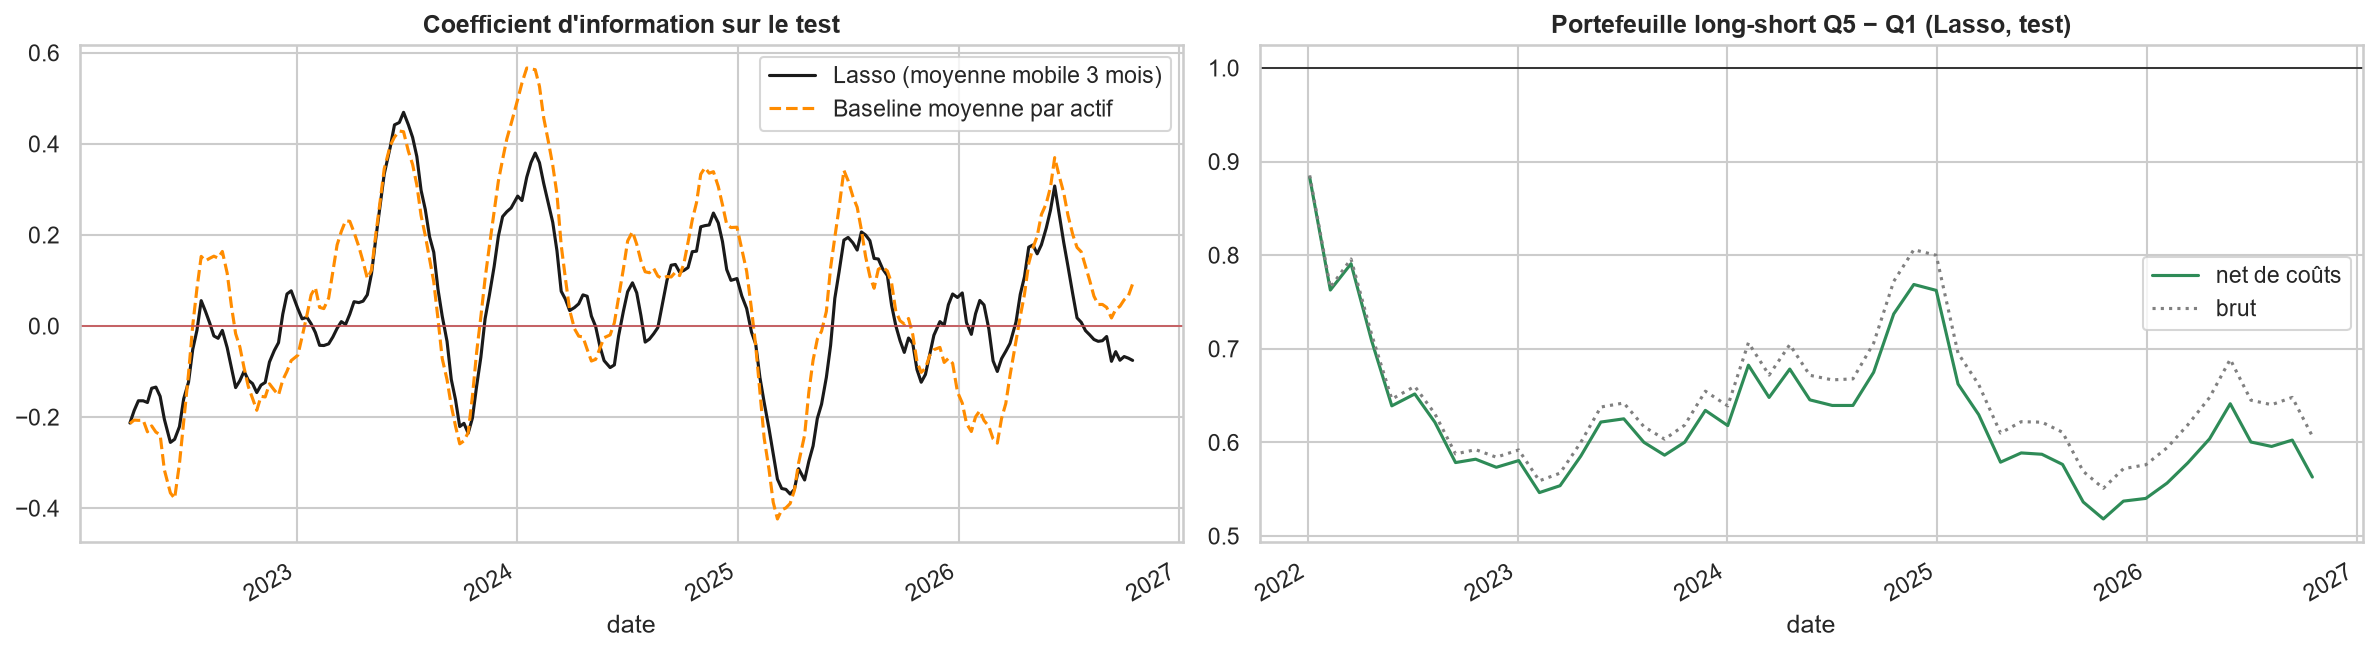
\includegraphics[width=\textwidth]{11_prevision_test.png}
  \caption{Sur le test : coefficient d'information (moyenne mobile sur trois mois) et valeur cumulée du portefeuille long-short Q5-Q1 construit avec l'ensemble.}
  \label{fig:prev_test}
\end{figure}

Ces résultats appellent trois commentaires.

\paragraph{La dérive des données s'est produite.} La référence \og moyenne par actif \fg{}, la meilleure sur 2013-2021, devient nettement moins bonne que la prévision nulle ($R^2 = -9{,}8$ \%). La prime de classe d'actifs s'est retournée en 2022, quand actions et obligations ont baissé ensemble. C'est exactement le risque annoncé par l'analyse exploratoire.

\paragraph{L'ensemble ne prévoit pas mieux les rendements.} Sa MSE est identique à celle de la prévision nulle ($R^2 = 0{,}15$ \%, $p = 0{,}94$). Le garde-fou a eu raison sur le critère qu'il s'était fixé.

\paragraph{Mais il classe un peu les actifs.} Son IC est de 0,10, significatif ($t = 2{,}35$), et le portefeuille long-short qui en découle gagne 9,8 \% par an après coûts. Faut-il en conclure qu'il aurait fallu l'activer ? Nous pensons que non, pour deux raisons. D'abord, l'IC a été très instable (négatif en 2022, autour de 0,17 de 2023 à 2025, proche de zéro en 2026) ; le simple momentum 12-1, sans apprentissage, fait presque aussi bien (9,4 \%). Ensuite, et surtout, changer la règle \emph{après} avoir vu le test reviendrait à utiliser le test pour décider : c'est précisément la fuite que tout notre protocole cherche à éviter. Le résultat est noté comme une piste : un critère fondé sur le classement (l'IC) plutôt que sur l'erreur quadratique pourrait être plus adapté à l'usage qu'on fait des prévisions. Il faudrait le valider sur une nouvelle période.

\subsection{Explicabilité et analyse des erreurs}

Les variables qui comptent le plus dans les prévisions (valeurs SHAP moyennes sur le test) sont les rendements passés à 3, 6 et 12 mois, le momentum 12-1 et les volatilités à 1 et 3 mois : le modèle combine un effet de tendance et un effet de risque. L'analyse par classe d'actifs montre que le modèle prévoit le bon \emph{sens} des écarts (rendement excédentaire prévu négatif pour les obligations et le monétaire, positif pour les actions et le Bitcoin) mais avec une amplitude bien plus faible que la réalité. C'est le comportement attendu d'un modèle fortement régularisé : il ramène ses prévisions vers zéro faute de confiance dans le signal.

En résumé, l'agent Prévision a été construit avec soin, évalué honnêtement et désactivé par une règle décidée à l'avance. Ce résultat négatif est, à nos yeux, l'un des apports du projet : il montre qu'un système d'apprentissage automatique doit savoir \emph{renoncer} à une prévision quand rien ne prouve qu'elle est utile.


\section{Agents Régime et Alerte : apprentissage non supervisé}
\label{sec:regime_alerte}

Les deux agents de cette section travaillent \emph{sans étiquette} : personne n'a écrit, jour après jour, si le marché était \og calme \fg{} ou \og anormal \fg{}. Ils relèvent donc de l'apprentissage non supervisé, et leur évaluation demande un soin particulier : en l'absence de vérité terrain, nous les jugeons sur des critères économiques fixés à l'avance.

\subsection{Agent Régime : objectif et variables}

L'agent Régime classe chaque journée en trois régimes : Calme, Neutre ou Stress. Ce régime sert à ajuster le risque du portefeuille et à informer le client. L'état du marché est décrit par cinq variables \textbf{stationnaires} : le rendement et le logarithme de la volatilité du S\&P~500 sur un mois, la perte depuis le plus haut sur un an, le logarithme du VIX et la variation sur trois mois du spread de crédit.

Ce choix de variables est le fruit d'un échec. La première version utilisait des \emph{niveaux} (pente de la courbe des taux, spread de crédit). La courbe s'étant inversée de 2022 à 2024, à un niveau jamais vu à l'entraînement, le modèle classait 91 \% du test en \og Stress \fg{}. Les logarithmes et les variations restent dans la plage observée pendant l'entraînement. Les modèles sont ajustés sur 2011-2019 (2\,391 jours), après une standardisation apprise sur cette période, puis appliqués date par date sans regarder le futur.

\subsection{Quatre familles de clustering}

Nous avons comparé les quatre familles de méthodes vues en cours (tableau~\ref{tab:clustering_methodes}).

\begin{table}[!htb]
  \centering
  \small
  \caption{Les quatre familles de clustering comparées.}
  \label{tab:clustering_methodes}
  \begin{tabularx}{\textwidth}{@{}l l L@{}}
    \toprule
    \textbf{Famille} & \textbf{Méthode} & \textbf{Principe} \\
    \midrule
    Partition & K-means & Minimise l'inertie intra-classe $J = \frac{1}{n}\sum_i \lVert x_i - \mu_{c(i)}\rVert^2$ \\
    Hiérarchique & CAH, critère de Ward~\cite{ward1963} & Fusionne à chaque étape les deux groupes dont la fusion augmente le moins l'inertie intra-classe \\
    Densité & DBSCAN~\cite{ester1996} & Un groupe est une zone dense ; les points isolés sont du bruit \\
    Probabiliste & Mélange gaussien, algorithme EM~\cite{dempster1977} & $p(x) = \sum_k \pi_k\,\mathcal{N}(x;\mu_k,\Sigma_k)$, estimé par maximum de vraisemblance \\
    \bottomrule
  \end{tabularx}
\end{table}

\paragraph{Nombre de régimes.} Le coude de K-means est peu marqué, et le critère BIC du mélange gaussien continue de baisser au-delà de trois groupes : avec 2\,400 jours, des groupes plus fins sont toujours un peu plus vraisemblables. Nous avons retenu \textbf{trois régimes}, nombre directement interprétable par un conseiller. Le cours le rappelle : le bon nombre de groupes est celui qui met en lumière une structure utile, pas seulement celui qui optimise un critère.

\paragraph{Règle de choix fixée à l'avance.} L'agent doit fournir des \emph{probabilités} d'appartenance aux régimes, affichées dans l'application et utilisables comme variables. Seul le mélange gaussien en produit : c'est lui que le système utilise. Les trois autres méthodes servent de comparaison et de contrôle de robustesse.

\begin{table}[!htb]
  \centering
  \small
  \caption{Qualité des partitions à trois groupes (entraînement). ARI : indice de Rand ajusté avec la partition du mélange gaussien. Pour DBSCAN, les indices excluent les 3,9 \% de points classés comme bruit.}
  \label{tab:clustering}
  \begin{tabular}{@{}l r r r r r@{}}
    \toprule
    \textbf{Méthode} & \textbf{Silhouette} $\uparrow$ & \textbf{Davies-Bouldin} $\downarrow$ & \textbf{Calinski-H.} $\uparrow$ & \textbf{Inertie expl.} & \textbf{ARI} \\
    \midrule
    K-means & 0,27 & 1,29 & 1\,451 & 55 \% & 0,27 \\
    CAH (Ward) & 0,36 & 1,18 & 1\,165 & 49 \% & 0,25 \\
    DBSCAN & 0,48 & 0,63 & 99 & 8 \% & 0,01 \\
    Mélange gaussien & 0,12 & 1,79 & 795 & 40 \% & 1 \\
    \bottomrule
  \end{tabular}
\end{table}

\paragraph{Interprétation.} Le tableau~\ref{tab:clustering} peut surprendre : la méthode retenue a les plus mauvais indices géométriques. C'est attendu, et c'est instructif. La silhouette~\cite{rousseeuw1987}, Davies-Bouldin et Calinski-Harabasz favorisent des groupes sphériques et bien séparés, ce que construit précisément K-means. Le mélange gaussien produit des \emph{ellipses qui se chevauchent}, avec une covariance propre à chaque régime. Il capte ainsi une structure que les autres méthodes ignorent : le régime de stress est beaucoup plus dispersé que le régime calme. Les bons scores de DBSCAN sont trompeurs : ils sont calculés sans les points classés comme bruit, ses groupes n'expliquent que 8 \% de l'inertie, et sa partition ne concorde pas avec celle des autres méthodes (ARI de 0,01~\cite{hubert1985}). Enfin, l'accord modéré entre K-means, CAH et mélange gaussien (ARI de 0,25 à 0,27) montre que les frontières entre régimes sont floues : le marché passe continûment du calme au stress. C'est un argument de plus pour des probabilités plutôt que des étiquettes tranchées. Le dendrogramme de la CAH figure en annexe (figure~\ref{fig:dendrogramme}).

\subsection{Description et validation économique des régimes}

Les trois régimes du mélange gaussien se décrivent simplement (tableau~\ref{tab:regimes}) et leurs différences sont toutes significatives (test de Kruskal-Wallis, $p < 10^{-4}$ pour chaque variable).

\begin{table}[!htb]
  \centering
  \small
  \caption{Description des régimes sur l'entraînement (moyennes).}
  \label{tab:regimes}
  \begin{tabular}{@{}l r r r r r@{}}
    \toprule
    \textbf{Régime} & \shortstack[r]{\textbf{Part}\\\textbf{des jours}} & \shortstack[r]{\textbf{Rendement}\\\textbf{1 mois}} & \textbf{Volatilité} & \shortstack[r]{\textbf{Perte depuis}\\\textbf{le plus haut}} & \textbf{VIX} \\
    \midrule
    Calme & 33 \% & $+2{,}9$ \% & 8,6 \% & $-0{,}2$ \% & 12,5 \\
    Neutre & 40 \% & $+0{,}5$ \% & 10,9 \% & $-1{,}8$ \% & 15,8 \\
    Stress & 27 \% & $+0{,}1$ \% & 18,4 \% & $-7{,}0$ \% & 21,1 \\
    \bottomrule
  \end{tabular}
\end{table}

Un bon régime ne doit pas seulement décrire le présent : il doit \emph{annoncer} le risque à venir. Nous mesurons donc la volatilité réalisée du S\&P~500 sur le mois qui suit chaque journée, et résumons le pouvoir informatif du découpage par le $\eta^2$, la part de la variance de cette volatilité future expliquée par le régime.

\begin{table}[!htb]
  \centering
  \small
  \caption{Volatilité et rendement du S\&P~500 sur le mois qui suit, selon le régime détecté. Les chiffres du test sont descriptifs et n'ont servi à aucun choix.}
  \label{tab:regimes_validation}
  \footnotesize\setlength{\tabcolsep}{4pt}
  \begin{tabular}{@{}l r r r r r r@{}}
    \toprule
     & \multicolumn{2}{c}{\textbf{Entraînement} ($\eta^2 = 0{,}21$)} & \multicolumn{2}{c}{\textbf{Validation} ($\eta^2 = 0{,}12$)} & \multicolumn{2}{c}{\textbf{Test} ($\eta^2 = 0{,}29$)} \\
    \cmidrule(lr){2-3}\cmidrule(lr){4-5}\cmidrule(l){6-7}
    \textbf{Régime} & Vol. future & Rdt futur & Vol. future & Rdt futur & Vol. future & Rdt futur \\
    \midrule
    Calme & 9,7 \% & 0,7 \% & 20,2 \% & $-3{,}2$ \% & 11,5 \% & 0,7 \% \\
    Neutre & 12,3 \% & 1,0 \% & 14,5 \% & 1,5 \% & 12,8 \% & 1,1 \% \\
    Stress & 17,4 \% & 2,1 \% & 26,9 \% & 4,1 \% & 20,6 \% & 1,2 \% \\
    \bottomrule
  \end{tabular}
\end{table}

\begin{figure}[!htb]
  \centering
  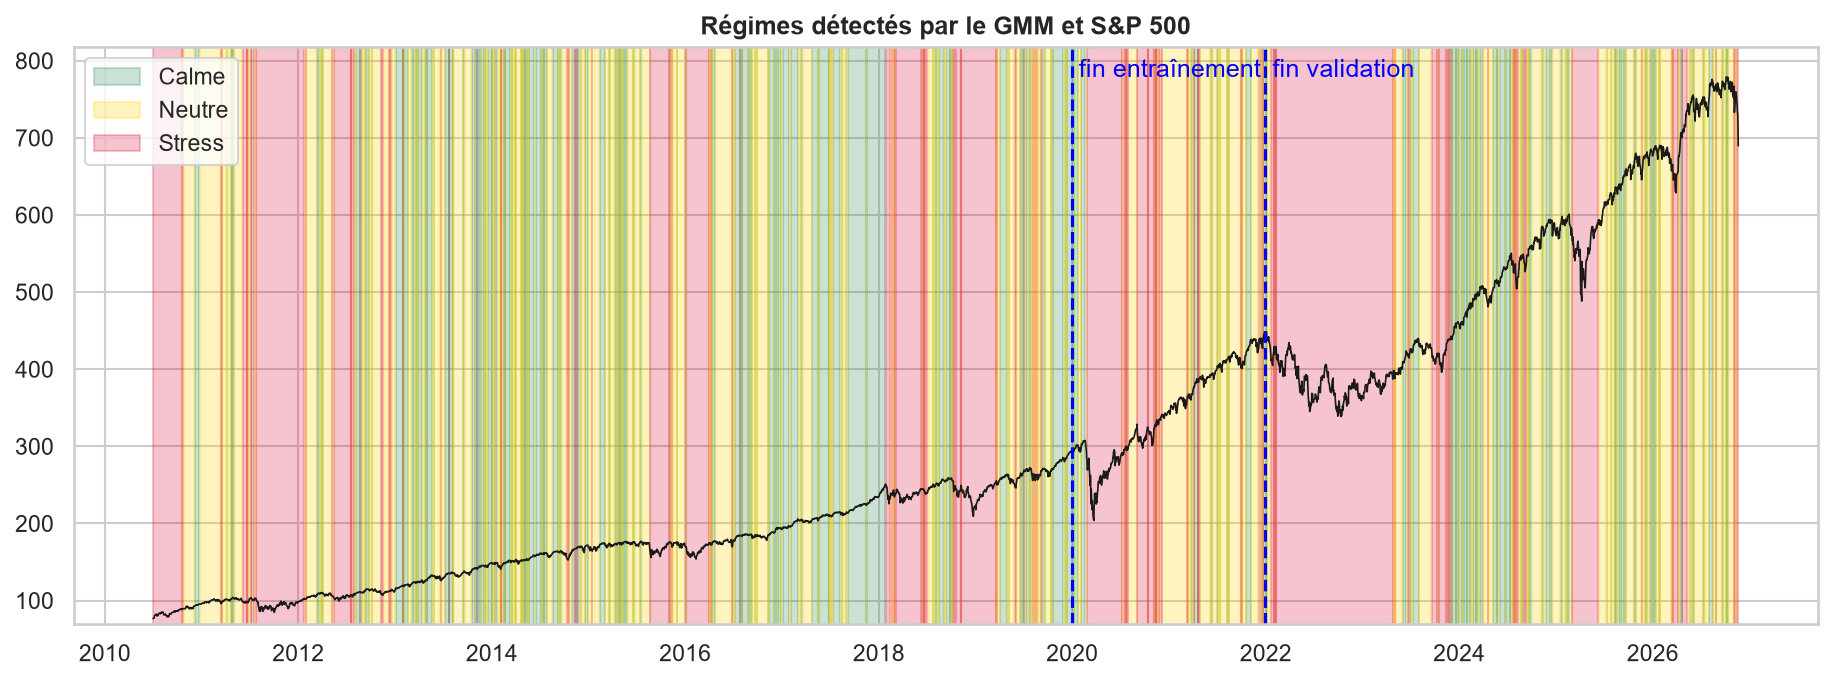
\includegraphics[width=\textwidth]{16_regimes.png}
  \caption{Régimes détectés par le mélange gaussien et cours du S\&P~500.}
  \label{fig:regimes}
\end{figure}

Trois enseignements se dégagent (tableau~\ref{tab:regimes_validation} et figure~\ref{fig:regimes}) :
\begin{itemize}
  \item \textbf{L'agent repère le risque.} Sur les trois périodes, le régime Stress est suivi de la volatilité la plus élevée, et le régime explique 12 à 29 \% de la variance de la volatilité future. Les régimes sont aussi très persistants (la matrice de transition a une diagonale proche de 1), ce qui rend leur détection en temps réel exploitable.
  \item \textbf{Il réagit au risque, il ne l'anticipe pas.} En validation, le régime Calme est suivi d'une volatilité \emph{plus forte} que le régime Neutre. C'est l'effet de février 2020 : le marché était parfaitement calme juste avant le krach de la COVID. Aucune variable de marché ne pouvait annoncer une pandémie ; l'agent bascule en Stress avec quelques jours de retard.
  \item \textbf{Il n'annonce pas de baisse.} Les périodes de stress ont plutôt été suivies de \emph{rebonds} (rendement futur moyen le plus élevé). Réduire systématiquement l'exposition en régime de stress ferait donc souvent vendre au mauvais moment. Ce point sera arbitré sur la validation lors du réglage de l'allocation (section~\ref{sec:allocation_backtest}).
\end{itemize}

\subsection{Les probabilités de régime comme variables de prévision}

Le cours présente une autre utilisation du mélange gaussien : ses probabilités a posteriori $\gamma_{ik}$, ou \og responsabilités \fg{}, peuvent servir de nouvelles variables pour un modèle supervisé. Nous les avons ajoutées aux variables de l'agent Prévision, dans l'idée que certains actifs réagissent différemment selon le régime, puis nous avons comparé les versions avec et sans ces variables par le test de Diebold-Mariano.

Le résultat est négatif. Pour Ridge, l'ajout ne change pas l'erreur de façon significative, ni sur la validation ($p = 0{,}10$) ni sur les prévisions hors pli ($p = 0{,}15$), et la statistique est même légèrement en défaveur de la version enrichie. Pour un arbre peu profond, les prévisions sont strictement identiques : l'arbre n'utilise aucune des trois nouvelles variables. L'information du régime est déjà contenue dans les variables de volatilité et le VIX. Le mélange gaussien sert donc à \emph{décrire} le marché et à gérer le risque, pas à prévoir les rendements relatifs.

\subsection{Agent Alerte : détection d'anomalies}

Une anomalie est une observation rare, qui se distingue nettement de la majorité des données. Ici, c'est une journée de marché anormale : krach, choc de liquidité. L'agent Alerte a deux usages : prévenir le conseiller et le client, et contrôler la qualité des données téléchargées. Nous avons comparé six méthodes du cours :
\begin{itemize}
  \item deux méthodes statistiques sur le rendement du S\&P~500 : le \textbf{z-score} (alerte au-delà de 4 écarts-types) et le \textbf{test de Grubbs}~\cite{grubbs1969}, répété tant qu'il rejette l'hypothèse que la valeur la plus extrême est normale ;
  \item quatre méthodes d'apprentissage sur les cinq variables de marché : la \textbf{gaussienne multivariée} (anomalie si la densité $p(x;\mu,\Sigma)$ est inférieure à un seuil $\epsilon$), l'\textbf{Isolation Forest}~\cite{liu2008} (une anomalie s'isole en peu de coupures aléatoires), le \textbf{LOF}~\cite{breunig2000} (densité locale nettement plus faible que celle des voisins) et la \textbf{One-Class SVM}~\cite{scholkopf2001} (frontière qui entoure les données normales).
\end{itemize}
Les paramètres sont appris sur 2011-2019, avec un taux d'anomalies attendu de 2 \%. L'alerte finale est un \textbf{vote} : elle n'est levée que si au moins trois des quatre méthodes d'apprentissage sont d'accord.

\paragraph{Validation sans étiquettes.} Il n'existe pas de liste officielle des journées anormales. Nous avons donc jugé les détecteurs sur deux critères : retrouvent-ils les crises connues, et s'accordent-ils entre eux ?

\begin{table}[!htb]
  \centering
  \small
  \caption{Détection de six crises connues ($\checkmark$ : au moins une alerte pendant l'épisode).}
  \label{tab:crises}
  \begin{tabular}{@{}l c c c c c c@{}}
    \toprule
    \textbf{Épisode} & \textbf{Gauss.} & \shortstack{\textbf{Isol.}\\\textbf{Forest}} & \textbf{LOF} & \shortstack{\textbf{One-Class}\\\textbf{SVM}} & \shortstack{\textbf{Vote}\\\textbf{$\geq 3/4$}} & \textbf{z-score} \\
    \midrule
    Crise de la dette, août 2011 & $\checkmark$ & $\checkmark$ & $\checkmark$ & $\checkmark$ & $\checkmark$ & $\checkmark$ \\
    Dévaluation du yuan, août 2015 & $\checkmark$ & $\checkmark$ & -- & $\checkmark$ & $\checkmark$ & $\checkmark$ \\
    \og Volmageddon \fg{}, février 2018 & $\checkmark$ & -- & $\checkmark$ & $\checkmark$ & $\checkmark$ & $\checkmark$ \\
    Krach de la COVID, mars 2020 & $\checkmark$ & $\checkmark$ & $\checkmark$ & $\checkmark$ & $\checkmark$ & $\checkmark$ \\
    Choc d'inflation, juin 2022 & $\checkmark$ & $\checkmark$ & $\checkmark$ & $\checkmark$ & $\checkmark$ & $\checkmark$ \\
    Choc de liquidité, août 2024 & $\checkmark$ & -- & $\checkmark$ & $\checkmark$ & $\checkmark$ & -- \\
    \bottomrule
  \end{tabular}
\end{table}

Le vote détecte \textbf{les six crises} (tableau~\ref{tab:crises}), alors que, prises isolément, seules la gaussienne et la One-Class SVM les détectent toutes. Les détecteurs multivariés s'accordent largement entre eux (corrélations de 0,41 à 0,80 entre leurs alertes). Le z-score, en revanche, leur est peu corrélé (0,09 à 0,27) : il repère les chocs brutaux d'une seule journée, alors que les méthodes multivariées repèrent des \emph{états} anormaux qui durent, quand volatilité, VIX et spread de crédit s'élèvent ensemble. Les deux approches sont complémentaires.

\begin{figure}[!htb]
  \centering
  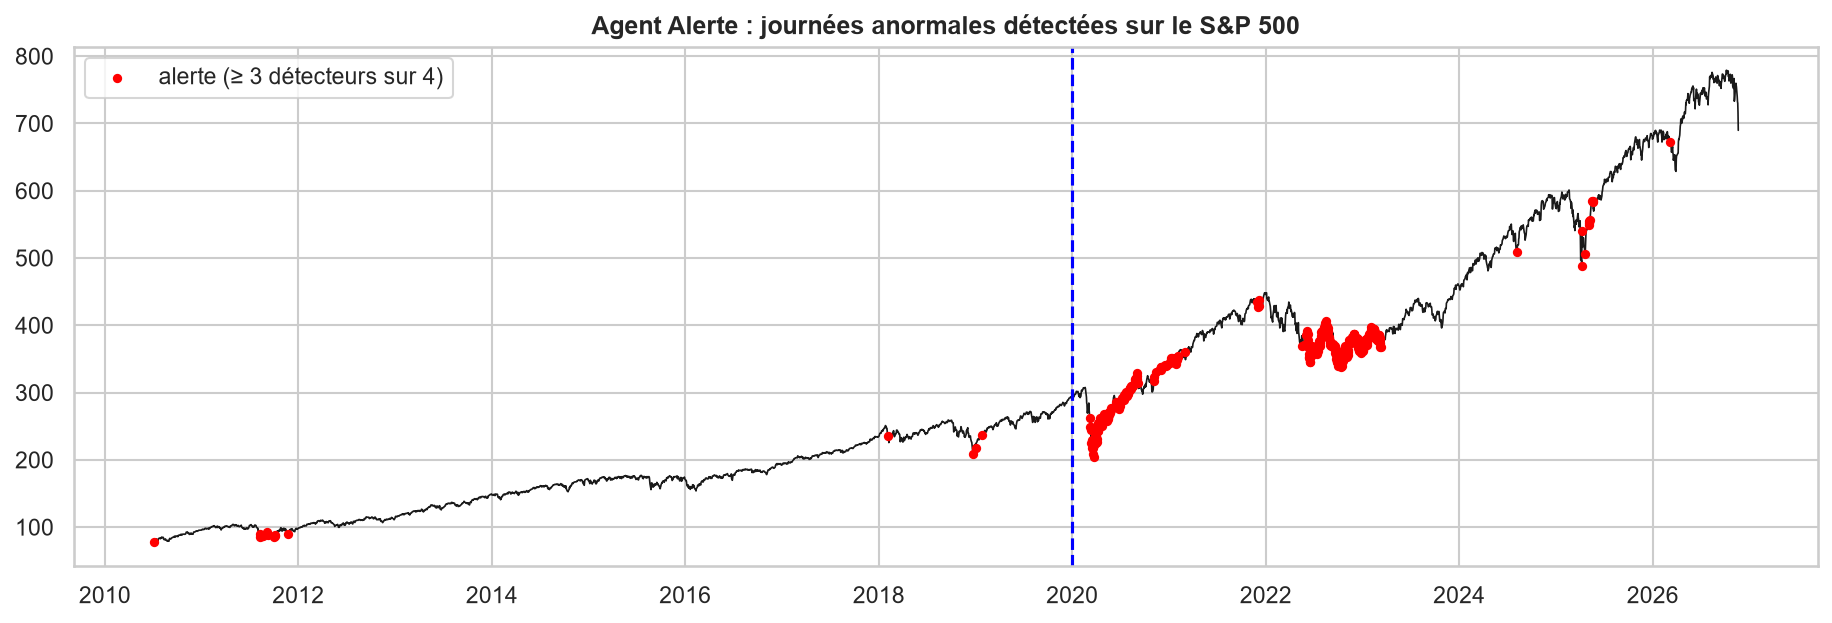
\includegraphics[width=\textwidth]{16b_anomalies.png}
  \caption{Journées signalées par le vote d'au moins trois détecteurs sur quatre. La ligne pointillée marque la fin de l'entraînement.}
  \label{fig:anomalies}
\end{figure}

\paragraph{La dérive des données, encore.} Le vote signale 0,6 \% des jours sur l'entraînement, mais 19 \% après 2019 (figure~\ref{fig:anomalies}) : 2020, puis 2022, ont été bien plus agités que les années 2010. Ce n'est pas une erreur du détecteur : c'est le marché qui a changé. Mais cela montre une limite de tout détecteur appris sur le passé. Pour éviter de banaliser les alertes, il faudrait recalibrer périodiquement les seuils sur des données récentes ; le vote à trois détecteurs sur quatre limite déjà les fausses alertes.

\section{Le système multi-agent}
\label{sec:systeme}

À rédiger.

\section{Allocation et évaluation historique}
\label{sec:allocation_backtest}

Un système de recommandation de portefeuille se juge, en dernier ressort, sur la performance des portefeuilles qu'il aurait recommandés. Cette section simule ces recommandations sur la période de test, avec un protocole qui interdit toute information future, et les compare à des stratégies simples de même risque.

\subsection{Protocole \emph{walk-forward}}

\begin{itemize}
  \item \textbf{Rebalancement mensuel}, le dernier jour de bourse de chaque mois, de janvier 2022 à novembre 2026 (60 rebalancements).
  \item À chaque date, la covariance est estimée sur les 252 jours précédents, et le régime avec les seules données disponibles.
  \item Entre deux rebalancements, les poids dérivent avec les prix ; les \textbf{coûts de transaction} (10 points de base par unité échangée) sont déduits à chaque rebalancement.
  \item Deux réglages ne sont appris par aucun modèle : la pénalité de rotation $\gamma$ et l'intensité de la réduction du risque en régime de stress. Ils sont choisis \textbf{sur la validation 2020-2021}, jamais sur le test.
\end{itemize}

\paragraph{Réglages choisis sur la validation.} Nous avons testé $\gamma \in \{0{,}5 ; 2 ; 5 ; 10\}$ et quatre intensités de réduction du risque en régime de stress (cible de volatilité multipliée par 1 ; 0,9 ; 0,75 ou 0,6), avec pour critère le ratio de Sharpe moyen des trois profils sur 2020-2021. Le choix retenu est $\gamma = 0{,}5$ et \textbf{aucune réduction}. Ce second résultat confirme la section~\ref{sec:regime_alerte} : les régimes de stress étant souvent suivis de rebonds, réduire le risque à ce moment fait vendre au mauvais moment. Le système garde l'agent Régime pour informer le client, mais ne s'en sert pas pour modifier l'allocation. C'est une décision guidée par les données, même si elle contredit l'intuition de départ.

\paragraph{Stratégies comparées.} Pour chaque profil, le système multi-agent est comparé à quatre références de risque comparable : son allocation stratégique de référence rebalancée chaque mois (sans optimisation) ; le 1/N, la parité de risque et HRP, chacun ramené à la volatilité cible du profil par un mélange avec la poche monétaire. Quatre références classiques complètent le tableau : 1/N brut, 60/40, variance minimale et Markowitz sur rendements historiques. Une limite doit être signalée : sans emprunt, on peut seulement \emph{réduire} le risque d'un portefeuille en ajoutant du monétaire. La parité de risque et HRP, naturellement peu risquées, restent donc en dessous des cibles des profils Équilibré et Dynamique ; pour ces profils, la comparaison porte sur le ratio de Sharpe plutôt que sur le rendement.

\subsection{Performances sur le test}

\begin{table}[!htb]
  \centering
  \small
  \caption{Performances sur le test (janvier 2022 à novembre 2026), nettes de coûts. Sharpe : rendement excédentaire au taux sans risque divisé par la volatilité. Rotation : somme des poids échangés par an.}
  \label{tab:backtest}
  \setlength{\tabcolsep}{5pt}
  \begin{tabular}{@{}l l r r r r r@{}}
    \toprule
    \textbf{Profil} & \textbf{Stratégie} & \textbf{Rendement} & \textbf{Volatilité} & \textbf{Sharpe} & \textbf{Perte max.} & \textbf{Rotation} \\
    \midrule
    \multirow{5}{*}{Prudent} & \textbf{Multi-agent} & \textbf{2,2 \%} & \textbf{6,3 \%} & $\boldsymbol{-0{,}26}$ & $\boldsymbol{-15{,}0}$ \textbf{\%} & \textbf{93 \%} \\
     & Référence stratégique & 3,2 \% & 7,4 \% & $-0{,}08$ & $-16{,}1$ \% & 46 \% \\
     & 1/N vol. cible & 4,8 \% & 6,9 \% & 0,13 & $-12{,}9$ \% & 81 \% \\
     & Parité de risque vol. cible & 4,1 \% & 6,6 \% & 0,04 & $-14{,}1$ \% & 90 \% \\
     & HRP vol. cible & 2,9 \% & 4,5 \% & $-0{,}23$ & $-11{,}1$ \% & 190 \% \\
    \midrule
    \multirow{5}{*}{Équilibré} & \textbf{Multi-agent} & \textbf{4,7 \%} & \textbf{9,6 \%} & \textbf{0,12} & $\boldsymbol{-18{,}2}$ \textbf{\%} & \textbf{74 \%} \\
     & Référence stratégique & 5,4 \% & 10,5 \% & 0,17 & $-18{,}6$ \% & 52 \% \\
     & 1/N vol. cible & 6,2 \% & 10,5 \% & 0,25 & $-18{,}0$ \% & 95 \% \\
     & Parité de risque vol. cible & 4,9 \% & 7,4 \% & 0,14 & $-15{,}1$ \% & 71 \% \\
     & HRP vol. cible & 2,8 \% & 4,6 \% & $-0{,}24$ & $-11{,}1$ \% & 194 \% \\
    \midrule
    \multirow{5}{*}{Dynamique} & \textbf{Multi-agent} & \textbf{8,1 \%} & \textbf{13,3 \%} & \textbf{0,35} & $\boldsymbol{-19{,}9}$ \textbf{\%} & \textbf{67 \%} \\
     & Référence stratégique & 8,3 \% & 13,7 \% & 0,36 & $-19{,}9$ \% & 58 \% \\
     & 1/N vol. cible & 7,1 \% & 11,7 \% & 0,30 & $-19{,}6$ \% & 61 \% \\
     & Parité de risque vol. cible & 4,9 \% & 7,4 \% & 0,14 & $-15{,}1$ \% & 70 \% \\
     & HRP vol. cible & 2,8 \% & 4,6 \% & $-0{,}24$ & $-11{,}1$ \% & 194 \% \\
    \midrule
    \multirow{4}{*}{--} & 1/N brut & 7,1 \% & 11,7 \% & 0,31 & $-19{,}6$ \% & 60 \% \\
     & 60/40 & 5,1 \% & 11,2 \% & 0,15 & $-20{,}9$ \% & 39 \% \\
     & Variance minimale & 1,3 \% & 4,9 \% & $-0{,}53$ & $-13{,}7$ \% & 111 \% \\
     & Markowitz historique & 17,0 \% & 19,5 \% & 0,70 & $-23{,}2$ \% & 616 \% \\
    \bottomrule
  \end{tabular}
\end{table}

\begin{figure}[!htb]
  \centering
  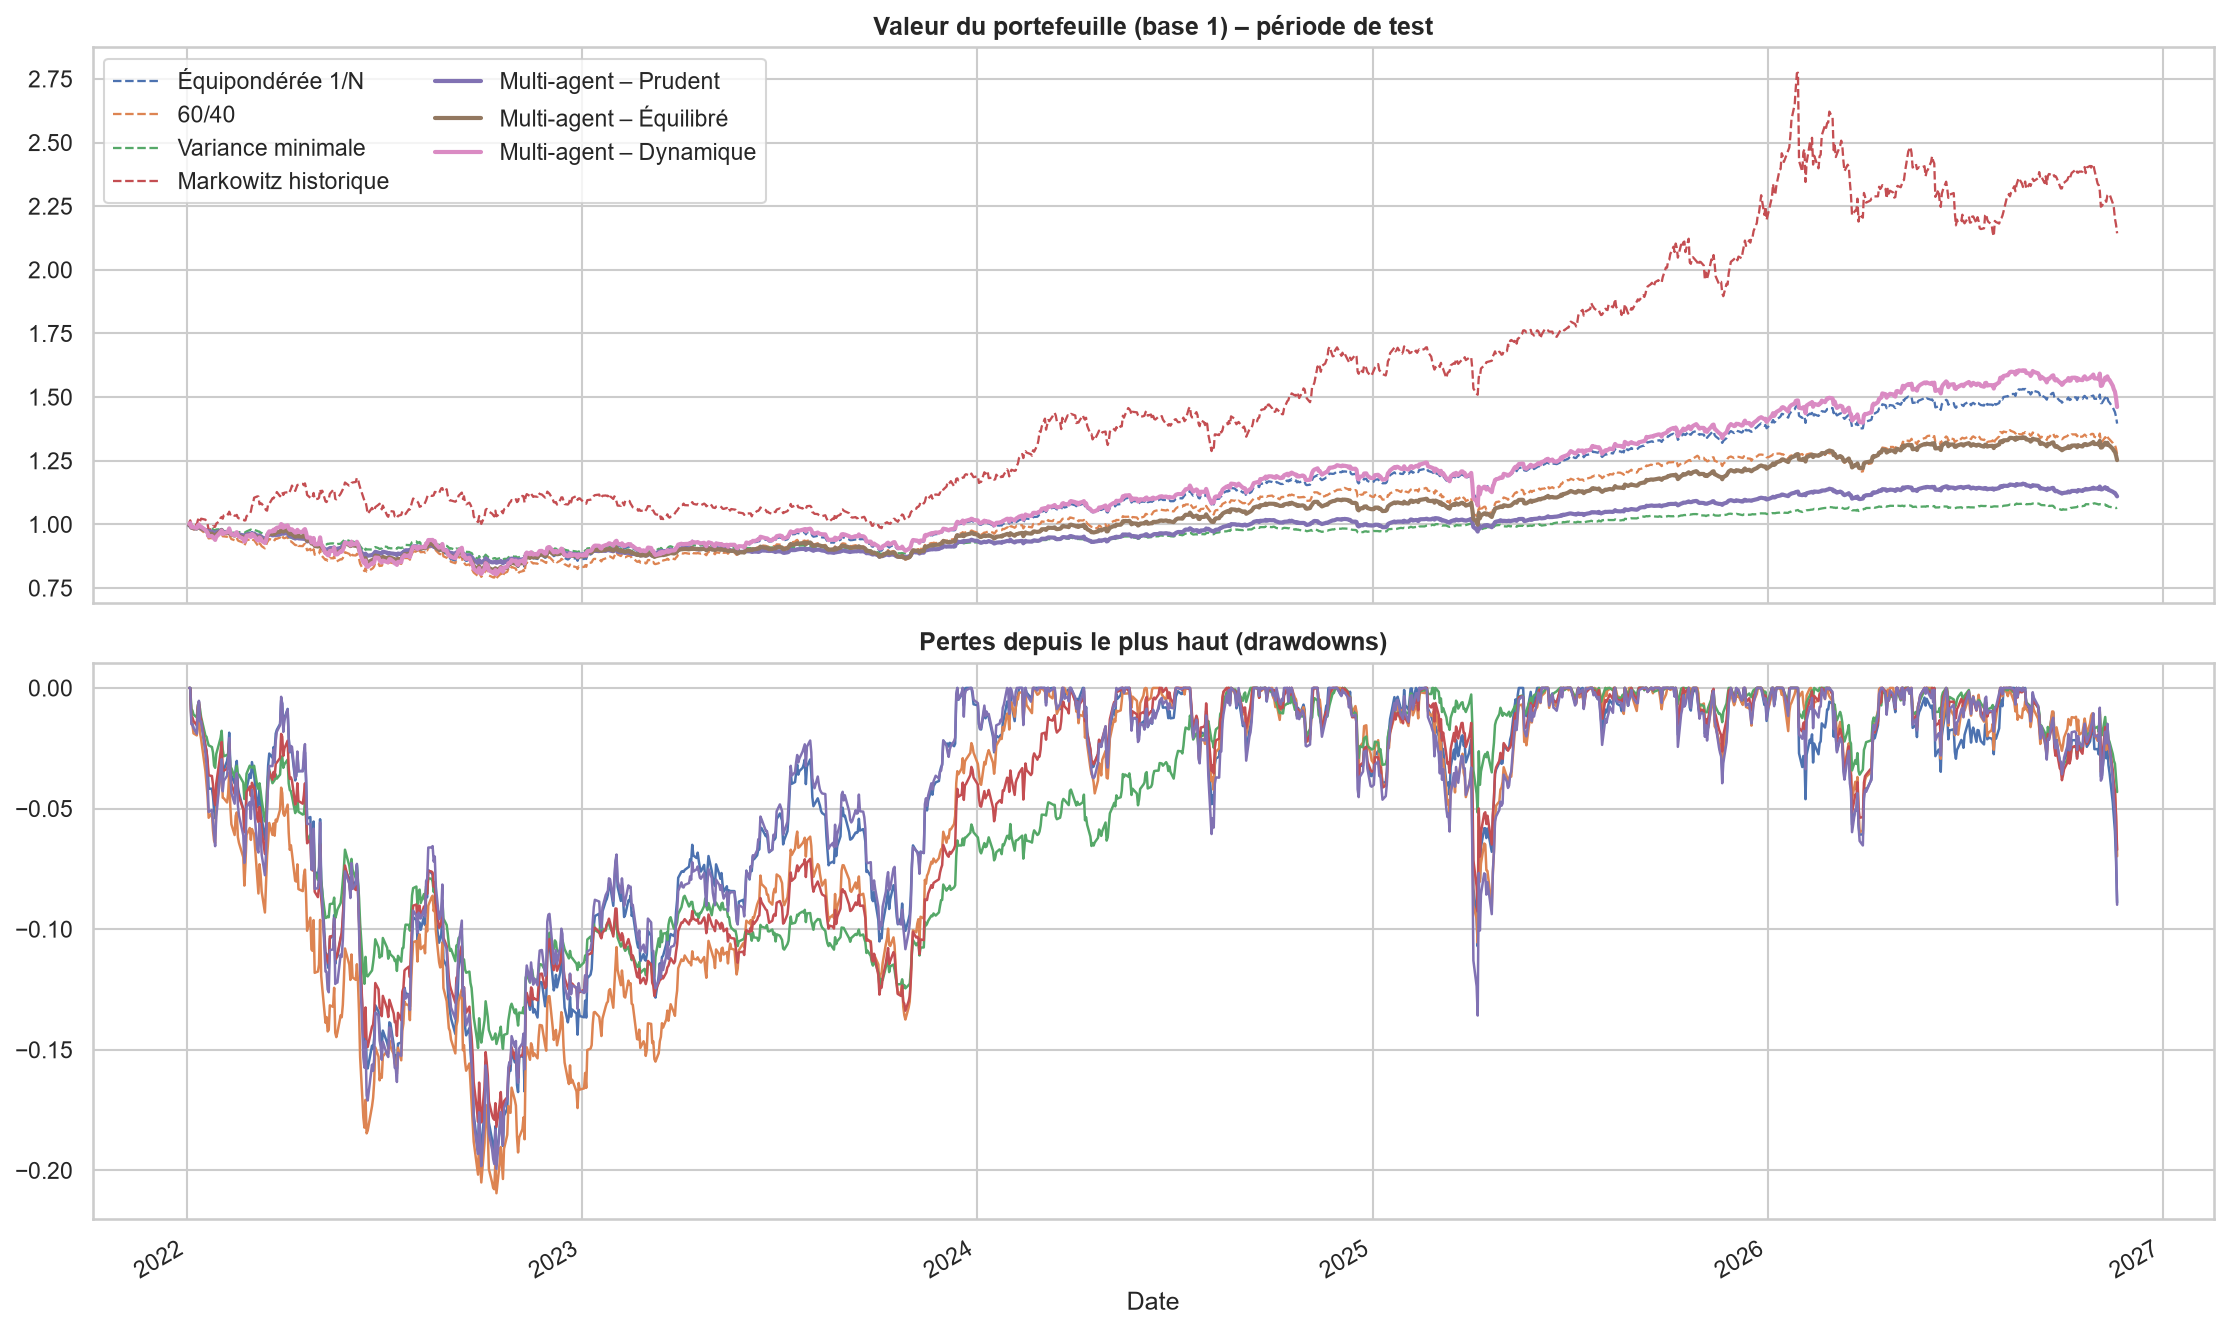
\includegraphics[width=\textwidth]{18_backtest_valeur_drawdown.png}
  \caption{Valeur des portefeuilles (base 1) et pertes depuis le plus haut sur la période de test.}
  \label{fig:backtest}
\end{figure}

\subsection{Significativité : bootstrap par blocs}

Sur moins de cinq ans, les écarts de ratio de Sharpe sont très bruités. Nous estimons un intervalle de confiance à 95 \% de la \emph{différence} de Sharpe entre le système et chaque référence par \textbf{bootstrap par blocs}~\cite{kunsch1989} : on rééchantillonne des blocs de 21 jours consécutifs, ce qui préserve l'autocorrélation et le regroupement de volatilité que détruirait un bootstrap ordinaire. Si l'intervalle contient zéro, la différence n'est pas établie.

\begin{table}[!htb]
  \centering
  \small
  \caption{Différence de Sharpe (multi-agent moins référence) et intervalle de confiance à 95 \% par bootstrap par blocs. En gras : différences significatives.}
  \label{tab:bootstrap}
  \begin{tabular}{@{}l r r r@{}}
    \toprule
    \textbf{Référence} & \textbf{Prudent} & \textbf{Équilibré} & \textbf{Dynamique} \\
    \midrule
    Référence stratégique & $-0{,}18$ \; [$-0{,}38$ ; 0,06] & $-0{,}06$ \; [$-0{,}15$ ; 0,06] & $-0{,}01$ \; [$-0{,}05$ ; 0,04] \\
    1/N vol. cible & $\boldsymbol{-0{,}39}$ \; [$-0{,}71$ ; $-0{,}13$] & $-0{,}13$ \; [$-0{,}37$ ; 0,05] & 0,05 \; [$-0{,}10$ ; 0,19] \\
    Parité de risque vol. cible & $\boldsymbol{-0{,}31}$ \; [$-0{,}55$ ; $-0{,}12$] & $-0{,}02$ \; [$-0{,}23$ ; 0,20] & 0,21 \; [$-0{,}07$ ; 0,54] \\
    HRP vol. cible & $-0{,}04$ \; [$-0{,}24$ ; 0,25] & \textbf{0,36} \; [0,04 ; 0,79] & \textbf{0,59} \; [0,13 ; 1,15] \\
    \bottomrule
  \end{tabular}
\end{table}

\subsection{Interprétation}

\paragraph{La première mission est remplie : le risque correspond au profil.} La volatilité réalisée croît du profil Prudent (6,3 \%) au profil Dynamique (13,3 \%), en restant dans le budget de chaque profil, et les pertes maximales s'ordonnent de la même façon. C'est ce que l'on attend d'abord d'un conseiller : ne pas exposer un client prudent à un risque qu'il ne peut pas supporter.

\paragraph{L'optimisation n'ajoute pas de rendement.} Pour les profils Équilibré et Dynamique, le système fait jeu égal avec sa référence stratégique et le 1/N de même risque : aucune différence n'est significative (tableau~\ref{tab:bootstrap}). Les deux différences favorables, face à HRP, sont à relativiser, car HRP est nettement moins risqué (4,6 \% de volatilité) : la comparaison n'est pas à risque égal.

\paragraph{Le profil Prudent est le point faible.} Il fait significativement moins bien que le 1/N et que la parité de risque de même volatilité. Sur 2022-2026, les portefeuilles prudents qui détenaient davantage d'actions diversifiées et moins d'obligations ont mieux traversé la hausse des taux de 2022. Notre contrainte de part défensive minimale (50 \%), même élargie au monétaire, a pesé. Ce n'est pas un défaut de l'optimiseur mais un choix de construction du profil, que l'on pourrait revoir ; il faudrait toutefois le faire sur une autre période que le test, pour ne pas ajuster le système au passé récent.

\paragraph{Pourquoi \og Markowitz historique \fg{} semble gagner.} Cette référence obtient de loin le meilleur Sharpe (0,70). Elle n'est pourtant pas un modèle à suivre : sa volatilité (19,5 \%) dépasse celle du profil Dynamique, et sa rotation de plus de 600 \% par an signifie qu'elle change presque entièrement de portefeuille tous les deux mois, en se concentrant sur les quelques actifs qui ont le plus monté récemment. Sur cette période, poursuivre les actifs en hausse a été payant ; dans un marché qui se retourne, la même concentration produit l'inverse. C'est exactement l'instabilité qui a conduit Black et Litterman à proposer leur a priori~\cite{black1992}. Sur une période différente, le classement pourrait être tout autre.

\paragraph{En résumé.} Nos résultats rejoignent ceux de la littérature : à risque égal, l'optimisation ne bat pas des règles simples~\cite{demiguel2009}. La valeur du système ne tient pas à une surperformance, que rien ne permet d'affirmer, mais à l'\textbf{adéquation au profil}, au \textbf{contrôle du risque} et à l'\textbf{explication} de chaque recommandation.

\section{Apprentissage par renforcement}
\label{sec:renforcement}

L'agent Allocation de la section~\ref{sec:systeme} résout un problème d'optimisation dont nous écrivons nous-mêmes l'objectif. L'apprentissage par renforcement propose une autre voie : laisser un agent \emph{apprendre} une politique d'allocation par essais et erreurs, en interagissant avec le marché. Le cours le présente précisément sur un exemple de gestion de portefeuille ; nous l'avons mis en œuvre comme alternative à l'optimiseur.

\subsection{Formulation}

À chaque pas de temps, l'agent observe un état $s_t$, choisit une action $a_t$ selon sa politique $\pi(a\mid s)$, reçoit une récompense $r_t$ et passe à l'état $s_{t+1}$. Il cherche la politique qui maximise la récompense cumulée actualisée $G_t = \sum_{k\geq 0} \gamma^k r_{t+k}$. Le tableau~\ref{tab:rl} décrit nos choix.

\begin{table}[!htb]
  \centering
  \small
  \caption{Formulation du problème d'apprentissage par renforcement.}
  \label{tab:rl}
  \begin{tabularx}{\textwidth}{@{}l L@{}}
    \toprule
    \textbf{Composante} & \textbf{Dans ce projet} \\
    \midrule
    Environnement & Le marché historique, rejoué mois par mois (environnement \texttt{Gymnasium} écrit pour le projet) \\
    État $s_t$ & 5 variables de régime, 3 probabilités de régime, rendements à 1 et 3 mois et volatilité à 3 mois de chaque classe d'actifs, poids actuels (25 nombres) \\
    Action $a_t$ & Répartition entre 5 classes d'actifs (actions, immobilier, obligations, monétaire, matières premières) \\
    Récompense $r_t$ & $\sum_j R_j - \frac{\lambda}{2}\sum_j R_j^2 - c\,\lVert w_t - w_{t-1}\rVert_1$ : rendement du mois, moins une pénalité de risque (aversion $\lambda$ du profil), moins les coûts de transaction \\
    Politique & Réseau de neurones à deux couches de 64 neurones, appris par PPO \\
    \bottomrule
  \end{tabularx}
\end{table}

\paragraph{L'algorithme PPO.} \emph{Proximal Policy Optimization}~\cite{schulman2017} appartient aux méthodes fondées sur la politique : le réseau reçoit l'état et renvoie directement une distribution de probabilité sur les actions. Le dilemme exploration-exploitation est géré par le caractère aléatoire de cette distribution pendant l'entraînement, où l'agent essaie des allocations variées ; la politique est ensuite utilisée de façon déterministe. PPO limite l'ampleur de chaque mise à jour de la politique, ce qui le rend plus stable que les méthodes de gradient de politique plus anciennes. Nous avons utilisé l'implémentation de \texttt{stable-baselines3}~\cite{raffin2021}.

\paragraph{Respect des contraintes.} L'action brute passe par une fonction \emph{softmax}, qui donne des poids positifs de somme 1, puis elle est \textbf{projetée} sur l'ensemble des allocations admissibles du profil (plafond d'actions, part défensive minimale, plafonds du monétaire et des matières premières). L'agent ne peut donc jamais proposer un portefeuille interdit.

\paragraph{Protocole.} L'agent est entraîné sur 2011-2019, par épisodes de 24 mois tirés au hasard ; la meilleure de deux graines aléatoires est choisie sur la validation 2020-2021 ; une seule évaluation est faite sur le test. La règle de décision est fixée à l'avance : PPO ne remplace l'optimiseur que s'il le bat significativement pour un profil.

\paragraph{Limites assumées.} L'entraînement ne dispose que d'environ 108 mois, très peu pour l'apprentissage par renforcement, qui consomme habituellement des millions d'interactions. Le Bitcoin est exclu, faute d'historique avant 2014. Enfin, le budget de volatilité n'est pas une contrainte stricte comme dans l'optimiseur : il est seulement \emph{pénalisé} dans la récompense.

\subsection{Résultats}

Sur la validation, les résultats sont flatteurs : ratio de Sharpe de 0,59 à 0,73 selon le profil et la graine. Mais la volatilité réalisée y atteint déjà 12 \% pour le profil Prudent, le double de sa cible, et 27 \% pour le profil Dynamique : la pénalité de risque ne suffit pas à tenir le budget.

\begin{table}[!htb]
  \centering
  \small
  \caption{Agent PPO sur le test, comparé au système multi-agent et au 1/N de même risque.}
  \label{tab:ppo}
  \begin{tabular}{@{}l l r r r r r@{}}
    \toprule
    \textbf{Profil} & \textbf{Stratégie} & \textbf{Rendement} & \textbf{Volatilité} & \textbf{Sharpe} & \textbf{Perte max.} & \textbf{Rotation} \\
    \midrule
    \multirow{3}{*}{Prudent} & PPO & 1,9 \% & 8,5 \% & $-0{,}20$ & $-18{,}8$ \% & 362 \% \\
     & Multi-agent & 2,2 \% & 6,3 \% & $-0{,}26$ & $-15{,}0$ \% & 93 \% \\
     & 1/N vol. cible & 4,8 \% & 6,9 \% & 0,13 & $-12{,}9$ \% & 81 \% \\
    \midrule
    \multirow{3}{*}{Équilibré} & PPO & 1,9 \% & 11,4 \% & $-0{,}12$ & $-23{,}5$ \% & 564 \% \\
     & Multi-agent & 4,7 \% & 9,6 \% & 0,12 & $-18{,}2$ \% & 74 \% \\
     & 1/N vol. cible & 6,2 \% & 10,5 \% & 0,25 & $-18{,}0$ \% & 95 \% \\
    \midrule
    \multirow{3}{*}{Dynamique} & PPO & 1,7 \% & 15,0 \% & $-0{,}08$ & $-28{,}4$ \% & 663 \% \\
     & Multi-agent & 8,1 \% & 13,3 \% & 0,35 & $-19{,}9$ \% & 67 \% \\
     & 1/N vol. cible & 7,1 \% & 11,7 \% & 0,30 & $-19{,}6$ \% & 61 \% \\
    \bottomrule
  \end{tabular}
\end{table}

Sur le test (tableau~\ref{tab:ppo}), l'agent PPO a un ratio de Sharpe négatif pour les trois profils. Le bootstrap par blocs montre qu'il fait significativement moins bien que le 1/N de même risque pour les trois profils, et que le système multi-agent pour le profil Dynamique (différence de Sharpe de $-0{,}43$, intervalle $[-0{,}84 ; -0{,}11]$). Il dépasse la volatilité cible de chaque profil, subit des pertes maximales plus fortes et échange de 3,6 à 6,6 fois son portefeuille par an, contre moins d'une fois pour l'optimiseur.

\paragraph{Interprétation.} Le passage de résultats flatteurs en validation à des résultats négatifs en test est le symptôme classique du \textbf{surapprentissage}. Avec une centaine de mois, l'agent a appris des régularités propres aux années 2010 (des actions qui montent, des obligations qui protègent), qui se sont retournées en 2022. Le choix de la graine sur la validation n'a pas suffi : avec si peu de données, la validation elle-même est une mesure bruitée. L'optimiseur moyenne-variance, dont la structure est imposée plutôt qu'apprise, est moins exposé à ce risque. Conformément à la règle fixée à l'avance, \textbf{l'application conserve l'optimiseur}, plus stable et plus facile à expliquer. L'agent PPO reste dans le projet comme démonstration de la méthode et de ses limites sur des données financières rares.

\section{Application web et déploiement}
\label{sec:application}

À rédiger.

\section{Discussion : pertinence, valeur ajoutée et limites}
\label{sec:discussion}

\subsection{Pertinence de la démarche}

\paragraph{Découper le problème plutôt que chercher un modèle unique.} Recommander un portefeuille mêle des questions de nature très différente : classer un client, décrire un marché, détecter un événement rare, prévoir des rendements, optimiser sous contraintes. Le découpage en agents nous a permis de traiter chacune avec la famille de méthodes adaptée, et surtout de l'\emph{évaluer} avec la métrique et la référence qui lui conviennent : rappel des Prudents pour le profil, Diebold-Mariano pour la prévision, volatilité future pour les régimes, crises connues pour les alertes, Sharpe à risque égal pour l'allocation. Un modèle unique de bout en bout aurait été impossible à juger avec cette finesse, et impossible à expliquer.

\paragraph{Une évaluation conçue pour pouvoir dire non.} Nous avons fixé avant chaque évaluation sur le test la règle qui déciderait de l'usage du modèle : seuil de rappel pour le profil, garde-fou de Diebold-Mariano pour la prévision, supériorité significative pour PPO. Ces règles ont joué contre nous à deux reprises (prévision et renforcement), et nous les avons respectées. C'est ce qui donne du crédit aux résultats positifs : quand nous disons que le modèle de profil généralise (AUC de 0,844 sur une autre vague d'enquête), ce n'est pas le fruit d'un choix fait après coup.

\paragraph{Des résultats cohérents avec la littérature.} Nos conclusions principales (un pouvoir prédictif sur les rendements faible et instable, une optimisation qui ne bat pas des règles simples de même risque, un renforcement qui surapprend sur peu de données) sont celles que la recherche en finance a établies~\cite{welch2008,demiguel2009,gu2020}. Cela ne les rend pas moins intéressantes : les retrouver avec notre propre protocole montre que celui-ci ne fabrique pas de faux positifs. Un projet qui aurait annoncé une prévision très performante des rendements aurait dû, au contraire, éveiller la méfiance.

\subsection{Valeur ajoutée}

Le système ne promet pas de battre le marché. Sa valeur se situe ailleurs, à cinq niveaux.
\begin{enumerate}
  \item \textbf{Une double vérification du profil.} Le croisement entre la tolérance déclarée et la capacité estimée sur 4\,595 ménages réels, avec une alerte en cas d'incohérence, répond à un vrai problème de conseil : un client qui surestime sa tolérance au risque. Le modèle repère quatre clients prudents sur cinq, et le conseiller garde la décision finale.
  \item \textbf{Un risque maîtrisé.} Les portefeuilles réalisent un risque conforme à chaque profil, sur une période difficile (marché baissier de 2022, remontée des taux). C'est la première exigence envers un conseiller.
  \item \textbf{Une explicabilité de bout en bout.} Chaque recommandation est accompagnée d'un texte, d'une décomposition SHAP du profil et du journal des décisions de chaque agent ; chaque modèle est documenté par une fiche et ses résultats d'évaluation. Le système peut toujours répondre à la question \og pourquoi ? \fg{}.
  \item \textbf{La capacité à renoncer.} Le garde-fou de l'agent Prévision est, à notre sens, l'apport le plus original. Un système qui sait désactiver un de ses propres modèles, quand rien ne prouve son utilité, est plus fiable qu'un système qui utilise tout ce qu'il a appris.
  \item \textbf{Un outil réel et reproductible.} Une application utilisable en ligne sans installation, qui respecte la confidentialité des visiteurs, et un dépôt qui permet de tout reproduire en une commande.
\end{enumerate}

\subsection{Limites}

Nous voyons sept limites principales, que nous préférons énoncer clairement.
\begin{enumerate}
  \item \textbf{La période de test avait déjà été consultée} lors des versions précédentes du projet. Notre protocole limite le risque que nos choix s'y soient adaptés, mais seule une nouvelle période, postérieure à la remise du projet, permettrait une évaluation entièrement vierge.
  \item \textbf{Un modèle de profil américain.} L'enquête SCF décrit des ménages américains. Appliquer le modèle à un client marocain, même en convertissant ses montants en dollars, suppose que la relation entre situation financière et prudence soit la même dans les deux pays, ce que nous n'avons pas pu vérifier faute de données publiques équivalentes.
  \item \textbf{Un questionnaire non calibré.} Les seuils du questionnaire (8 et 15 points sur 21) et ses plafonds sont fixés à dire d'expert, inspirés des pratiques réglementaires, et non appris sur des données.
  \item \textbf{Un univers d'actifs en dollars.} Les 25 actifs sont cotés aux États-Unis. Pour un investisseur marocain, le risque de change, la fiscalité et l'accès à ces fonds ne sont pas pris en compte.
  \item \textbf{Le point faible du profil Prudent.} La contrainte de 50 \% d'actifs défensifs a coûté cher en 2022. Elle reflète une convention de la profession plus qu'une optimisation ; la revoir demanderait une autre période de validation.
  \item \textbf{Des détecteurs qui vieillissent.} La part de jours en alerte passe de 0,6 \% à 19 \% après 2019 : appris sur les années 2010, les détecteurs devront être recalibrés régulièrement.
  \item \textbf{Un historique court.} Une quinzaine d'années de données mensuelles, c'est peu pour des modèles flexibles, et c'est la cause principale de l'échec de l'agent PPO.
\end{enumerate}
Enfin, certaines méthodes ont été volontairement laissées hors du périmètre : réseaux récurrents de type LSTM, modèles de langage pour rédiger les explications, apprentissage semi-supervisé. Avec un signal aussi faible et si peu de données, nous avons jugé plus utile d'approfondir l'évaluation des méthodes du cours que d'en multiplier le nombre.

\section{Conclusion, perspectives et apprentissages}
\label{sec:conclusion}

\subsection{Conclusion}

Nous avons construit un assistant de sélection de portefeuille fondé sur sept agents spécialisés, qui mobilisent l'ensemble des familles de méthodes du cours : classification supervisée avec correction du déséquilibre des classes, régression sur données temporelles avec réduction de dimension, clustering, détection d'anomalies, apprentissage par renforcement et explicabilité. Chaque agent a été comparé à des références simples et évalué avec un protocole qui interdit les fuites de données.

Les résultats sont contrastés, et nous les avons présentés comme tels :
\begin{itemize}
  \item l'agent \textbf{Profil} fonctionne : une régression logistique, aussi performante que des modèles bien plus complexes, repère 80 \% des clients prudents et généralise à une autre vague d'enquête (AUC de 0,867 sur le test, 0,843 en validation externe) ;
  \item les agents \textbf{Régime} et \textbf{Alerte} décrivent utilement le marché : le régime de stress annonce une volatilité plus forte, et le vote des détecteurs retrouve les six crises connues ;
  \item l'agent \textbf{Prévision} ne bat pas la prévision nulle : il est désactivé par un garde-fou décidé à l'avance, ce que le test a confirmé ;
  \item l'\textbf{allocation} respecte le risque de chaque profil mais ne bat pas des règles simples de même risque, et l'agent de \textbf{renforcement} surapprend ;
  \item l'\textbf{application}, utilisable en ligne et en local, rend chaque recommandation explicable et traçable.
\end{itemize}
La valeur du système tient donc moins à une performance financière qu'à la qualité du conseil : un profil vérifié, un risque maîtrisé, des décisions expliquées, et la capacité de renoncer à un modèle qui n'a pas fait ses preuves.

\subsection{Perspectives}

Plusieurs prolongements nous paraissent prometteurs :
\begin{itemize}
  \item \textbf{Juger la prévision sur le classement.} Sur le test, l'agent Prévision classait correctement les actifs (IC de 0,10) sans réduire l'erreur quadratique. Un garde-fou fondé sur l'IC, plus proche de l'usage que l'allocation fait des prévisions, mériterait d'être évalué, sur une période nouvelle.
  \item \textbf{Adapter le système au contexte marocain} : actifs de la Bourse de Casablanca, prise en compte du dirham et du risque de change, et, si des données le permettaient, un modèle de profil appris sur des ménages marocains.
  \item \textbf{Calibrer le questionnaire} sur des données, par exemple en apprenant ses seuils à partir des réponses de clients réels.
  \item \textbf{Recalibrer automatiquement} les détecteurs d'anomalies et les régimes sur une fenêtre glissante, pour suivre la dérive des données.
  \item \textbf{Enrichir l'apprentissage par renforcement} par des données simulées (bootstrap de trajectoires de marché) pour compenser le faible nombre de mois historiques.
  \item \textbf{Réévaluer le système en conditions réelles} : la mise à jour quotidienne de la version en ligne accumule désormais une période vraiment nouvelle, sur laquelle le système pourra être jugé sans aucun biais.
\end{itemize}

\subsection{Ce que ce projet nous a appris}

Au-delà des résultats, ce projet a profondément changé notre manière d'aborder l'apprentissage automatique.

\paragraph{Sur la méthode.} Nous avons appris que l'évaluation compte autant que le modèle. Le moment le plus marquant a été de voir des modèles qui semblaient prédictifs sur la validation (un $R^2$ de 4 \%) devenir inutiles en validation croisée : un seul découpage nous aurait trompés. Nous avons appris à commencer par une référence simple, à séparer les données avant toute transformation, à placer chaque étape dans un pipeline, à respecter l'ordre du temps, et à tester statistiquement nos comparaisons plutôt que de nous fier à quelques millièmes d'écart. Nous avons surtout appris à fixer nos règles de décision \emph{avant} de voir les résultats, et à les appliquer même quand elles nous donnaient tort.

\paragraph{Sur les données réelles.} Les données réelles ne ressemblent pas aux exemples de cours. Il a fallu gérer des calendriers différents, des imputations multiples, des publications décalées dans le temps, des valeurs extrêmes qui ne sont pas des erreurs, et surtout des données dont la distribution change : la dérive de 2022 a affecté presque tous nos agents. Nous avons aussi appris à nos dépens qu'une variable mal choisie (un niveau plutôt qu'une variation) peut ruiner un modèle hors échantillon.

\paragraph{Sur la valeur des résultats négatifs.} Nous espérions, au début du projet, un modèle qui prévoit les marchés. Nous terminons avec un garde-fou qui le désactive, et nous en sommes plus fiers que d'un résultat spectaculaire. Savoir dire, preuves à l'appui, \og ce modèle n'apporte rien \fg{} est une compétence essentielle pour un ingénieur, et c'est celle que ce projet nous a le plus fait travailler.

\paragraph{Sur l'explicabilité.} Expliquer un modèle à un client oblige à le comprendre soi-même. Choisir une régression logistique plutôt qu'un ensemble d'arbres à performance égale nous a permis de produire des explications exactes, et même de recalculer le modèle dans un navigateur. Nous avons compris que la simplicité est souvent un choix d'ingénieur, pas un renoncement.

\paragraph{Sur l'ingénierie.} Passer d'un notebook à une application utilisable nous a confrontés à des questions que le cours ne traite pas directement : organisation du code en modules réutilisables, gestion des versions avec Git, conception d'une API, interface web, déploiement gratuit et respectueux de la vie privée, tests d'égalité entre deux implémentations, mise à jour automatique des données. Nous avons appris à avancer par petites étapes vérifiées, chacune testée et enregistrée avant de passer à la suivante.

\paragraph{Sur le travail en équipe.} Enfin, un projet de cette taille nous a appris à répartir le travail entre agents comme entre personnes : définir clairement ce que chaque partie reçoit et produit, se mettre d'accord sur les conventions, et relire le travail des autres. L'architecture multi-agent du système a, en quelque sorte, reflété notre propre organisation.


% ================================================================ Références
\clearpage
\markboth{RÉFÉRENCES}{Références}
\printbibliography[title=Références]

% ================================================================ Annexes
\clearpage
\appendix
\section{Annexe : tableaux détaillés}

À rédiger.


\end{document}
